%%%%%%%%%%%%%%%%%%%%%%%%%%%%%%%%%%%%%%%%%%  不使用 authblk 包制作标题  %%%%%%%%%%%%%%%%%%%%%%%%%%%%%%%%%%%%%%%%%%%%%%
%-------------------------------PPT Title-------------------------------------
\title{浅谈:~人工智能、材料基因工程与数字孪生}
%-----------------------------------------------------------------------------

%----------------------------Author & Date------------------------------------
\author[]{\vskip +10pt 姜\;\;骏\inst{}} %[]{} (optional, use only with lots of authors)
%% - Give the names in the same order as the appear in the paper.
%% - Use the \inst{?} command only if the authors have different
%%   affiliation.
\institute[BCC]{\inst{}%
%\institute[Gain~Strong]{\inst{}%
\vskip -15pt 北京市计算中心}
%\vskip -20pt {\large 格致斯创~科技}}
\date[\today] % (optional, should be abbreviation of conference name)
{	{\fontsize{6.2pt}{4.2pt}\selectfont{\textcolor{blue}{E-mail:~}\url{jiangjun@bcc.ac.cn}}}
\vskip 45 pt {\fontsize{8.2pt}{6.2pt}\selectfont{%清华大学\;\;物理系% 报告地点
	\vskip 5 pt \textrm{2025.02}}}
}

%% - Either use conference name or its abbreviation
%% - Not really information to the audience, more for people (including
%%   yourself) who are reading the slides onlin%%   yourself) who are reading the slides onlin%%   yourself) who are reading the slides onlineee
%%%%%%%%%%%%%%%%%%%%%%%%%%%%%%%%%%%%%%%%%%%%%%%%%%%%%%%%%%%%%%%%%%%%%%%%%%%%%%%%%%%%%%%%%%%%%%%%%%%%%%%%%%%%%%%%%%%%%

\subject{}
% This is only inserted into the PDF information catalog. Can be left
% out.
%\maketitle
\frame
{
%	\frametitle{\fontsize{9.5pt}{5.2pt}\selectfont{\textcolor{orange}{“高通量并发式材料计算算法与软件”年度检查}}}
\titlepage
}
%-----------------------------------------------------------------------------

%------------------------------------------------------------------------------列出全文 outline ---------------------------------------------------------------------------------
\section*{}
\frame[allowframebreaks]
{
	\frametitle{\textrm{Outline}}
%  \frametitle{\textcolor{mycolor}{\secname}}
  \tableofcontents%[current,currentsection,currentsubsection]
}
%在每个section之前列出全部Outline
%类似的在每个subsection之前列出全部Outline是\AtBeginSubsection[]
%\AtBeginSection[]
%{
%  \frame<handout:0>%[allowframebreaks]
%  {
%    \frametitle{Outline}
%%全部Outline中,本部分加亮
%    \tableofcontents[current,currentsection]
%  }
%}

%-----------------------------------------------PPT main Body------------------------------------------------------------------------------------
\small
\section{什么是人工智能}
\begin{frame}{人工智能的定义}
  \begin{itemize}
	  \item 人工智能\textrm{(AI)}:~让机器模拟人类智能的科学
	  \item \textrm{Turing}测试:~判断机器是否智能的标准~\textrm{(1950)}
	  \item 强~\textrm{AI} \textrm{vs.} 弱\textrm{AI}
		  \vskip 2pt
    \begin{itemize}
	    \item 强\textrm{AI}:~具有自主意识的机器(尚未实现)
	    \item 弱\textrm{AI}:~专用领域智能(当前主流)
    \end{itemize}
  \end{itemize}
\begin{figure}[h!]
\vspace*{-0.10in}
\centering
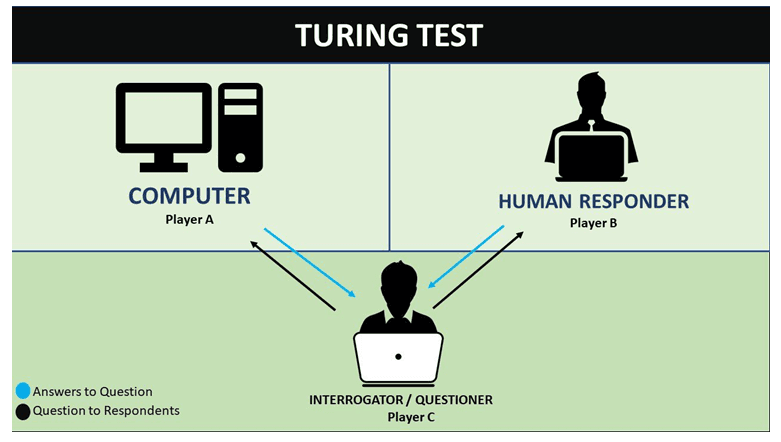
\includegraphics[height=1.55in, width=3.2in, viewport=0 0 2250 1230,clip]{Figures/The_Turing-Test.png}
%\caption{\tiny \textrm{Pseudopotential for metallic sodium, based on the empty core model and screened by the Thomas-Fermi dielectric function.}}%(与文献\cite{EPJB33-47_2003}图1对比)
\label{Turing_TEST}
\end{figure}
\end{frame}

%\section{发展历程}
\begin{frame}{历史里程碑}
%  \begin{columns}
 %   \column{0.5\textwidth}
%    \begin{itemize}
%	    \item \textrm{1956:~Dartmouth}会议
%	    \item \textrm{1997:~Deep-Blue}击败\textrm{Garry Kasparov}
 %     \item \textrm{2016:~Alpha~Go}战胜李世石
  %    \item \textrm{2022:~ChatGPT}发布
  %    \item \textrm{2025:~DeepSeek}发布
  %  \end{itemize}
%
%    \column{0.5\textwidth}
\begin{figure}[h!]
\vspace*{-0.10in}
\centering
   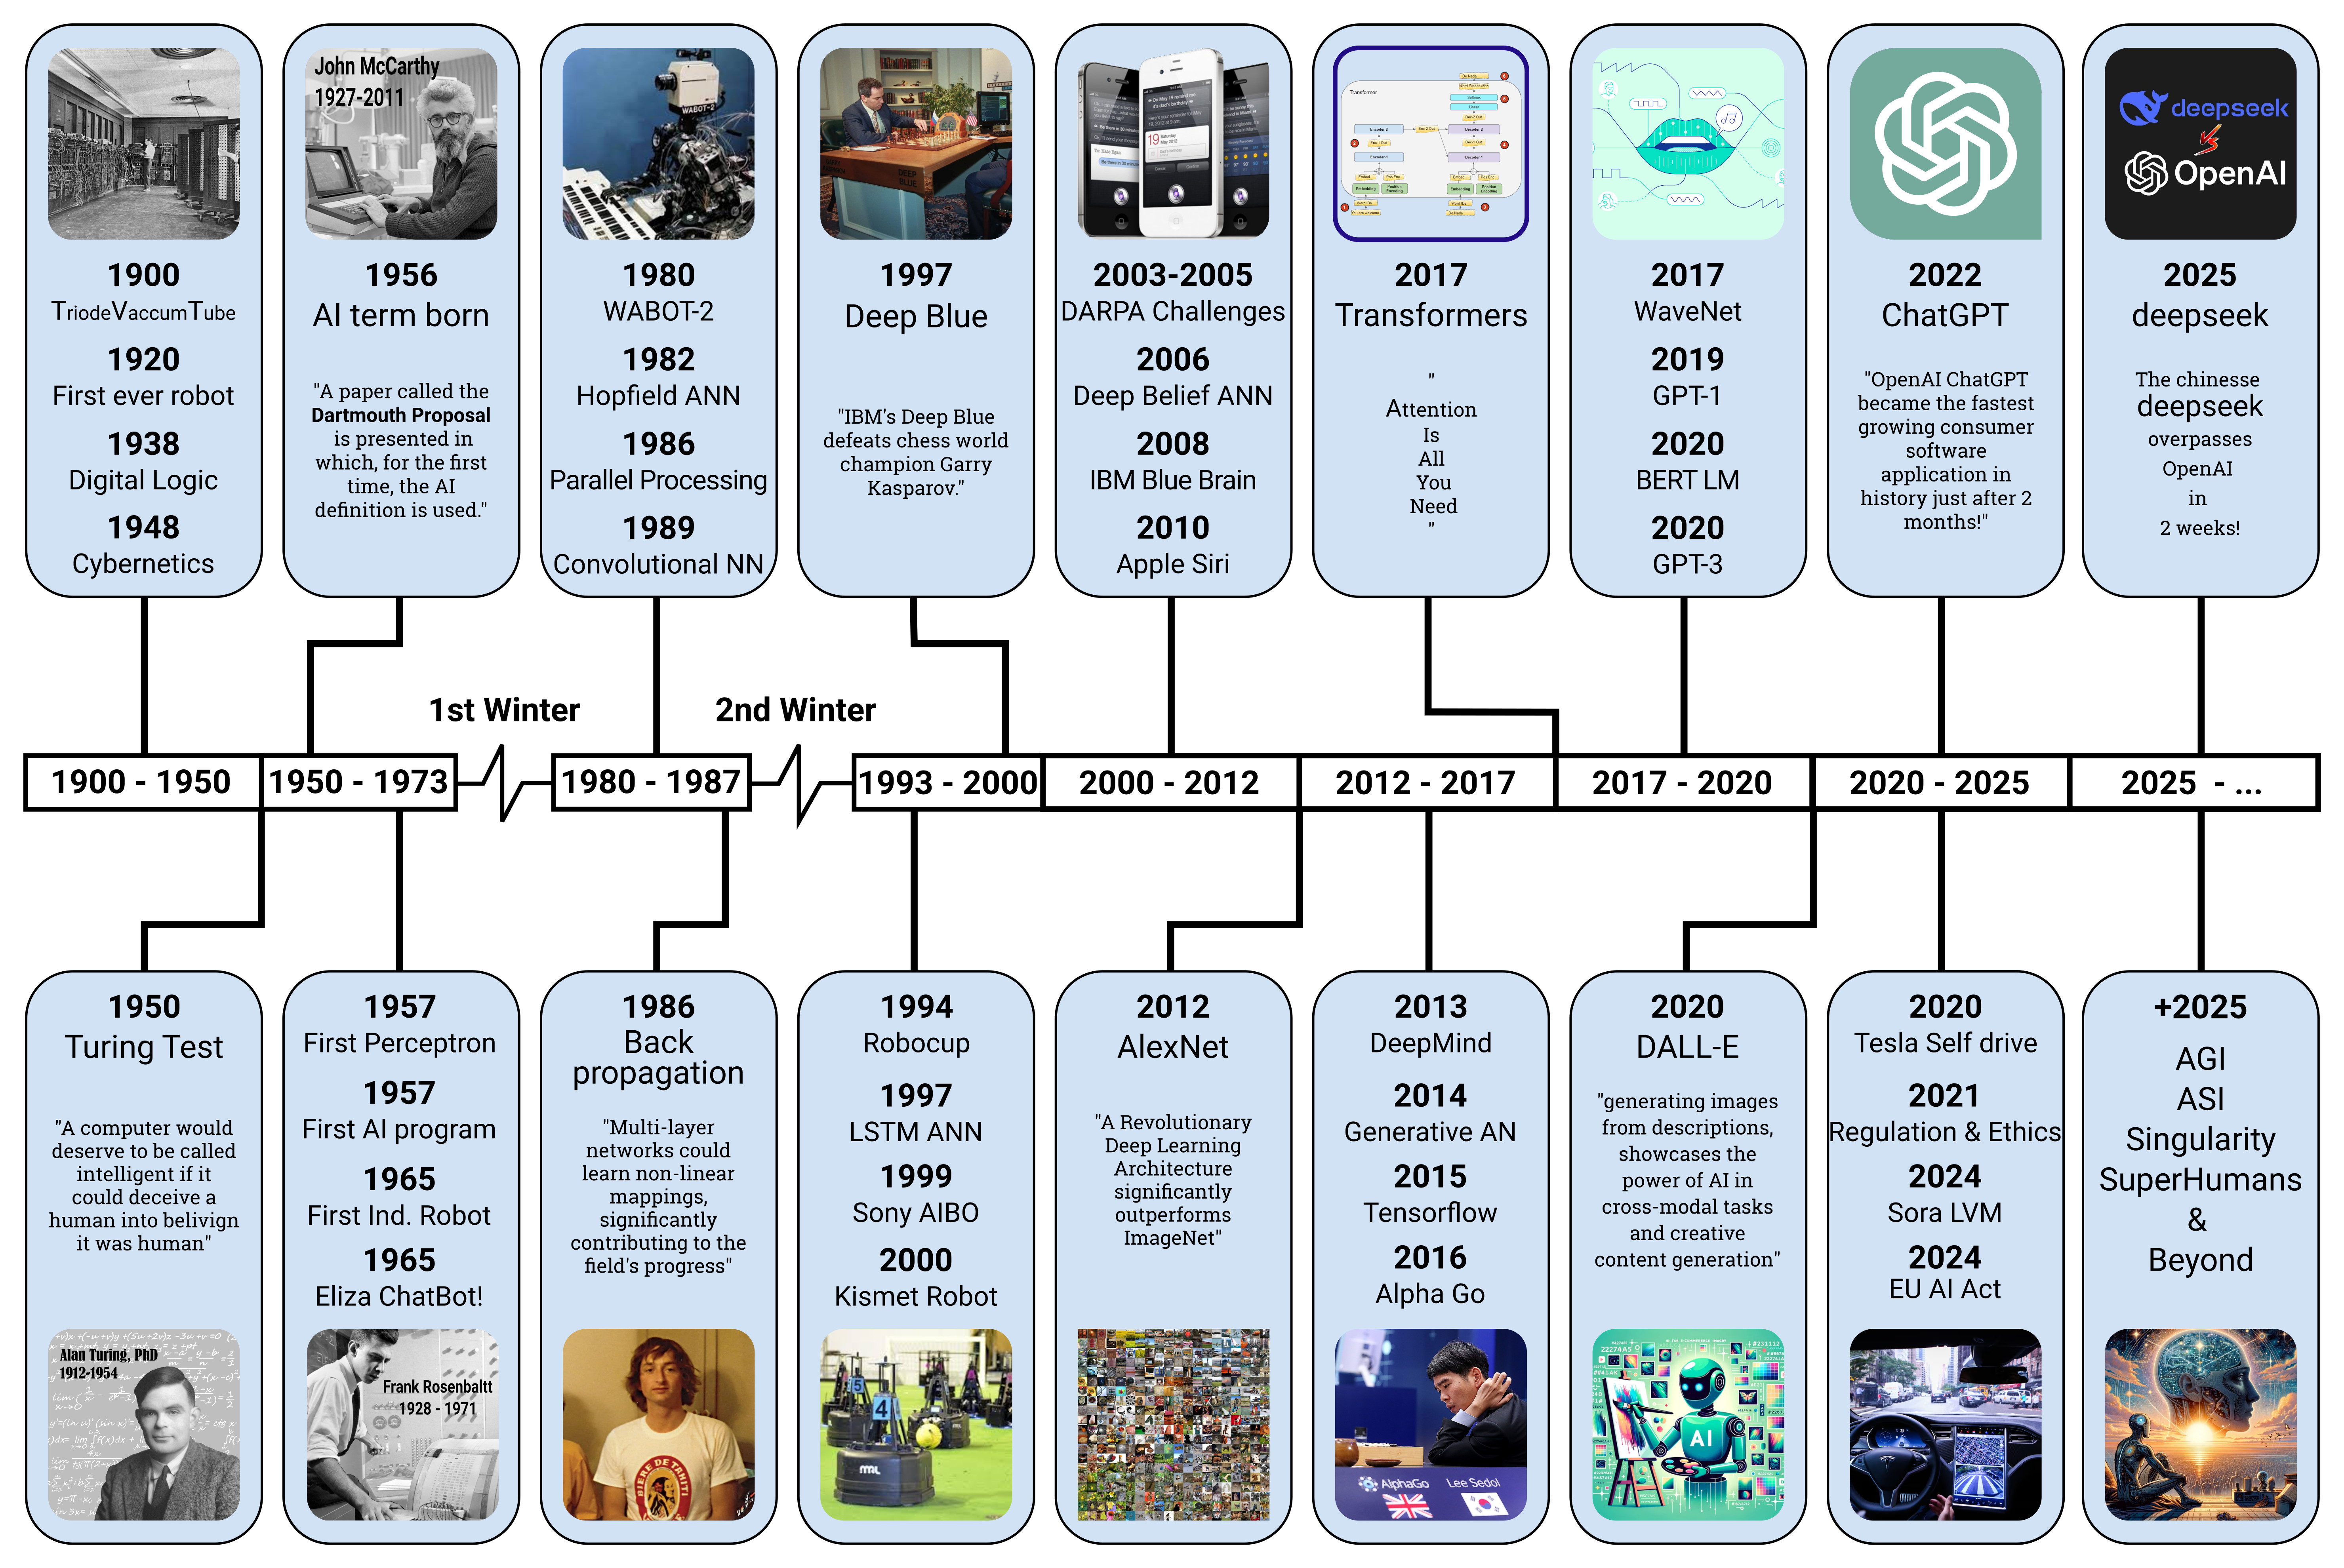
\includegraphics[width=\textwidth]{Figures/AI-History_timeline.jpg}
\label{AI-History}
\end{figure}
%  \end{columns}
\end{frame}

%\section{核心技术}
\subsection{机器学习}
\begin{frame}{机器学习基础}
  \begin{block}{机器学习的核心思想}
    从数据中自动学习规律
  \end{block}

  \begin{example}
    \begin{equation*}
      y = w \cdot x + b
    \end{equation*}
  \end{example}
  \begin{columns}
    \column{0.3\textwidth}
机器学习的分类
  \begin{itemize}
    \item 监督学习\\(分类/回归)
    \item 无监督学习\\(聚类)
    \item 强化学习\\(奖励机制)
  \end{itemize}
    \column{0.7\textwidth}
\begin{figure}[h!]
\vspace*{-0.45in}
\centering
   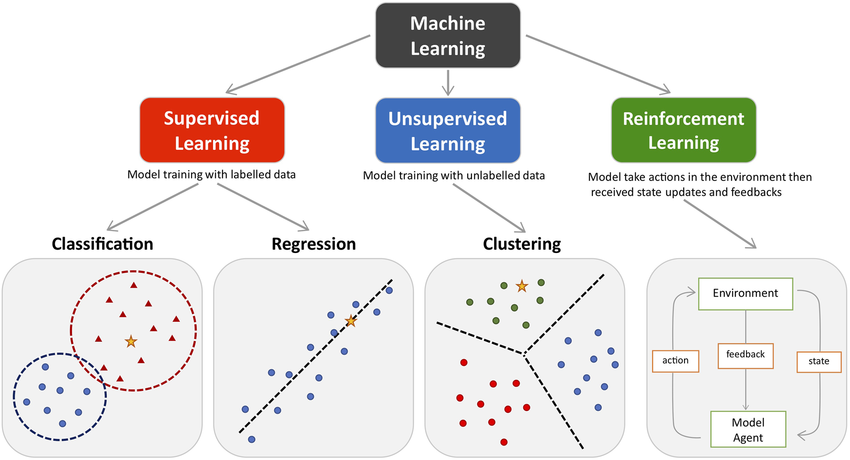
\includegraphics[height=1.6in, width=2.9in, viewport=0 0 210 120,clip]{Figures/The_main-types-of-machine-learning.png}
\label{Machine-Learning-types}
\end{figure}
  \end{columns}
\end{frame}

\subsection{深度学习}
\frame
{
	\frametitle{简单神经网络}
{\fontsize{8.0pt}{4.2pt}\selectfont{
	\begin{itemize}
		\item 感知机(\textrm{Perceptron Learning Algorithm, PLA}):
			\vskip 3pt
			最早的监督式训练算法,是神经网络构建的基础
\begin{figure}[h!]
%\vspace*{-0.08in}
\centering
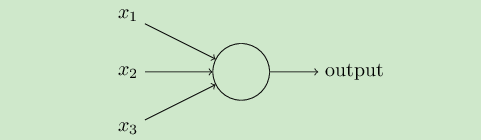
\includegraphics[height=0.50in]{Figures/DNN_PLA.png}
\caption{\tiny \textrm{Perceptron Learning Algorithm.}}%(与文献\cite{EPJB33-47_2003}图1对比)
\label{Fig:PLA}
\end{figure}
输出与输入之间将学习到一个线性关系,可有\textcolor{blue}{中间输出结果}
\begin{displaymath}
	z=\sum_{i=1}^mw_ix_i+b
\end{displaymath}
\textcolor{blue}{中间结}果连接一个神经元激活函数
\begin{displaymath}
	\mathrm{sign}(z)=\left\{
		\begin{aligned}
			-1\qquad &z<0\\
			1 \qquad &z\geqslant 0
		\end{aligned}\right.
\end{displaymath}
	\end{itemize}}}
}

\frame
{
	\frametitle{简单神经网络}
\begin{figure}[h!]
\vspace*{-0.08in}
\centering
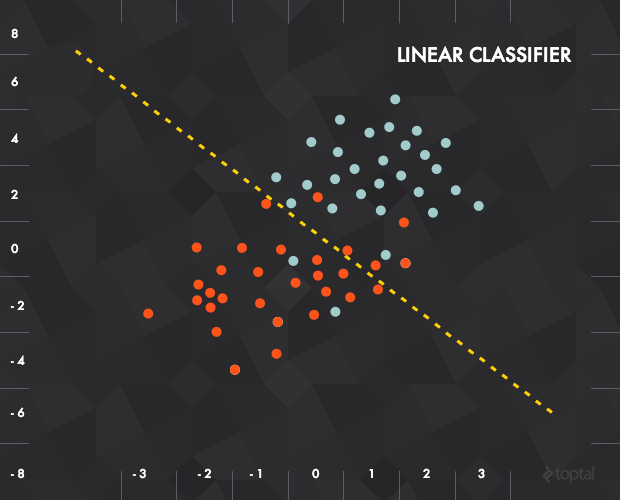
\includegraphics[width=2.5in]{Figures/NN_PLA_example.png}
%\caption{\tiny \textrm{Perceptron Learning Algorithm.}}%(与文献\cite{EPJB33-47_2003}图1对比)
\label{Fig:PLA_example}
\end{figure}
{\fontsize{8.0pt}{4.2pt}\selectfont{
\begin{itemize}
	\item 每一个输入数据都可以表示为一个向量$x = (x_1, x_2)$
	\item 函数则是要实现“如果线以下,输出0;线以上,输出1”
\end{itemize}}}
}

\frame
{
	\frametitle{深度神经网络基础}
{\fontsize{8.0pt}{4.2pt}\selectfont{
感知机模型只能用于二元分类,无法学习较为复杂的非线性模型,神经网络在感知机模型基础上作了扩展
%\vskip 10pt
	\begin{itemize}
		\item 加入隐藏层(\textrm{hide layer}):\\
			隐藏层可以有很多层,增强模型的表达能力
		\item 输出层的神经元可以有不止一个输出
		\item 对激活函数作扩展,如\textrm{Sigmoid}函数:~
			%\begin{displaymath}
				$f(z)=\dfrac1{1+\mathrm{e}^{-z}}$
			%\end{displaymath}
			\\{\fontsize{6.5pt}{4.2pt}\selectfont{其他的激活函数还有\textrm{tanx}、\textrm{softmax}和\textrm{ReLU}等}}
\begin{figure}[h!]
%\vspace*{-0.08in}
\centering
%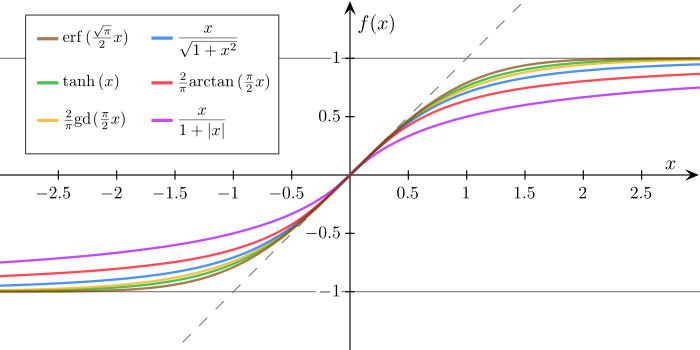
\includegraphics[width=2.8in]{Figures/ML_Sigmoid-Gjl-t.png}
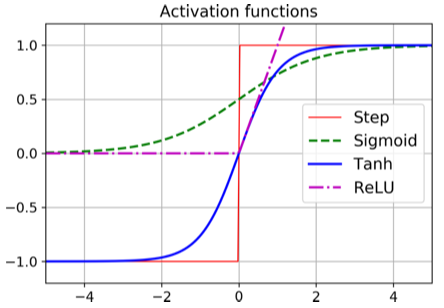
\includegraphics[width=2.3in]{Figures/ML_activation-function.png}
%\caption{\tiny \textrm{Perceptron Learning Algorithm.}}%(与文献\cite{EPJB33-47_2003}图1对比)
\label{Fig:Sigmoid_curve}
\end{figure}
	\end{itemize}}}
}

\frame
{
	\frametitle{深度神经网络}
%{\fontsize{8.0pt}{4.2pt}\selectfont{
深度神经网络可以包含上百层神经元,通常有上万个参数,再加上超参数,实际的参数空间几乎是无限大的%}}
\begin{figure}[h!]
%\vspace*{0.05in}
\centering
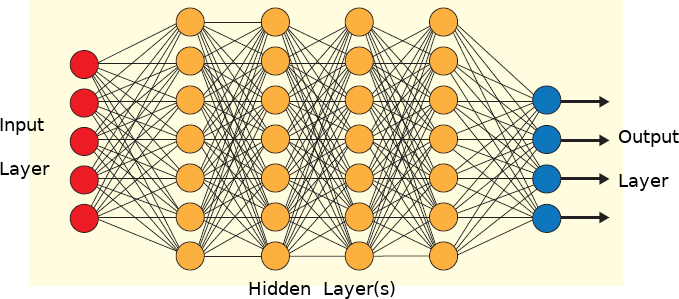
\includegraphics[height=1.90in,width=4.05in]{Figures/ANN_Algorithm.png}
\caption{\tiny \textrm{Deep Learning Neural Network.}}%(与文献\cite{EPJB33-47_2003}图1对比)
\label{Fig:Deep-Learning-NN}
\end{figure}
}
%\begin{frame}[fragile]{神经网络}
%  \begin{columns}
%    \column{0.4\textwidth}
%    \begin{itemize}
%      \item 模仿人脑神经元结构
%      \item 多层感知机\textrm{(MLP)}
%      \item 激活函数:~\textrm{ReLU,~Sigmoid}
%    \end{itemize}
%
%    \column{0.6\textwidth}
%    \begin{minted}{python}
%# 简单神经网络示例
%model = Sequential()
%model.add(Dense(64, activation='relu'))
%model.add(Dense(10, activation='softmax'))
%    \end{minted}
%  \end{columns}
%\end{frame}

\subsection{应用领域}
\begin{frame}{典型应用}
  \begin{itemize}
	  \item \textrm{AI}是通过机器学习模仿人类智能的技术
    \item 深度学习推动突破性进展
    \item 在多个领域产生革命性影响
%    \item 需要重视伦理规范和社会影响
  \end{itemize}

  \begin{columns}
    \column{0.33\textwidth}
    \centering
    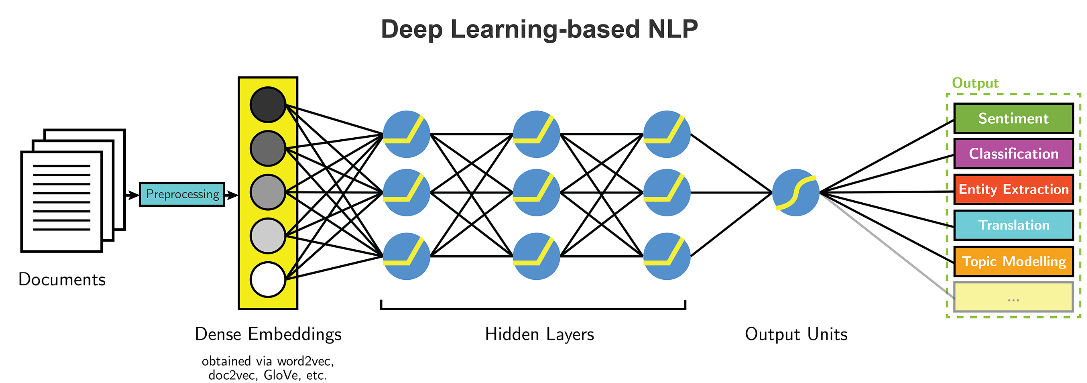
\includegraphics[width=0.8\textwidth]{Figures/AI_Deeplearning-NLP.png}\\
    自然语言处理

    \column{0.33\textwidth}
    \centering
    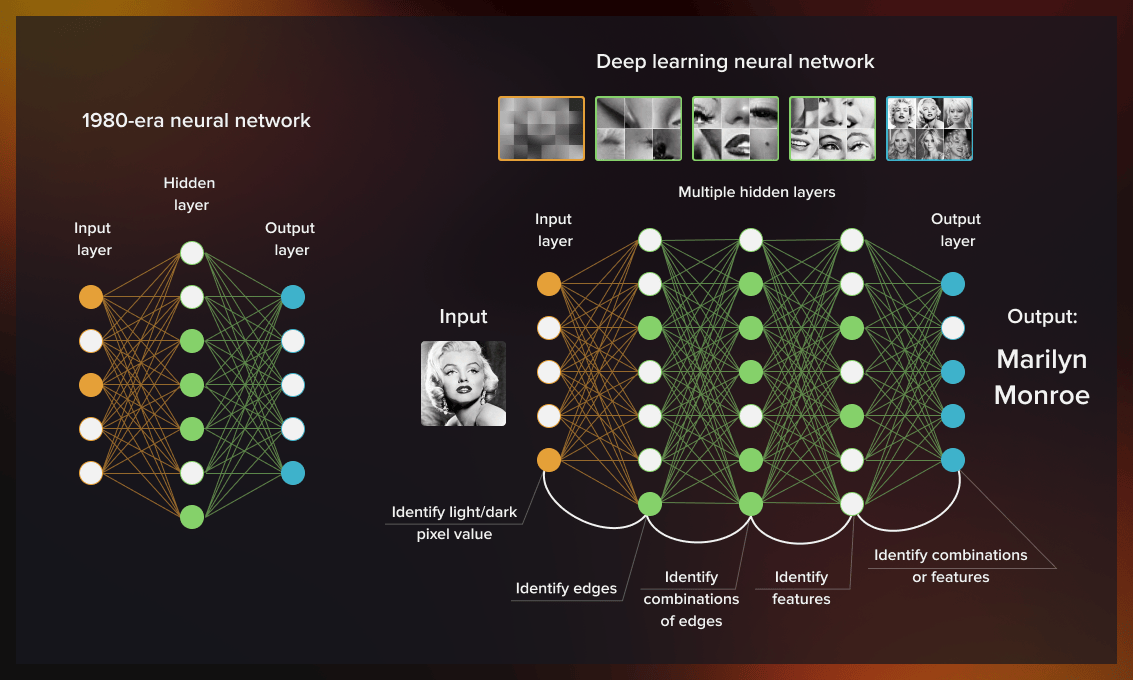
\includegraphics[width=0.8\textwidth]{Figures/AI_Deeplearning-CV.png}\\
    计算机视觉

    \column{0.33\textwidth}
    \centering
    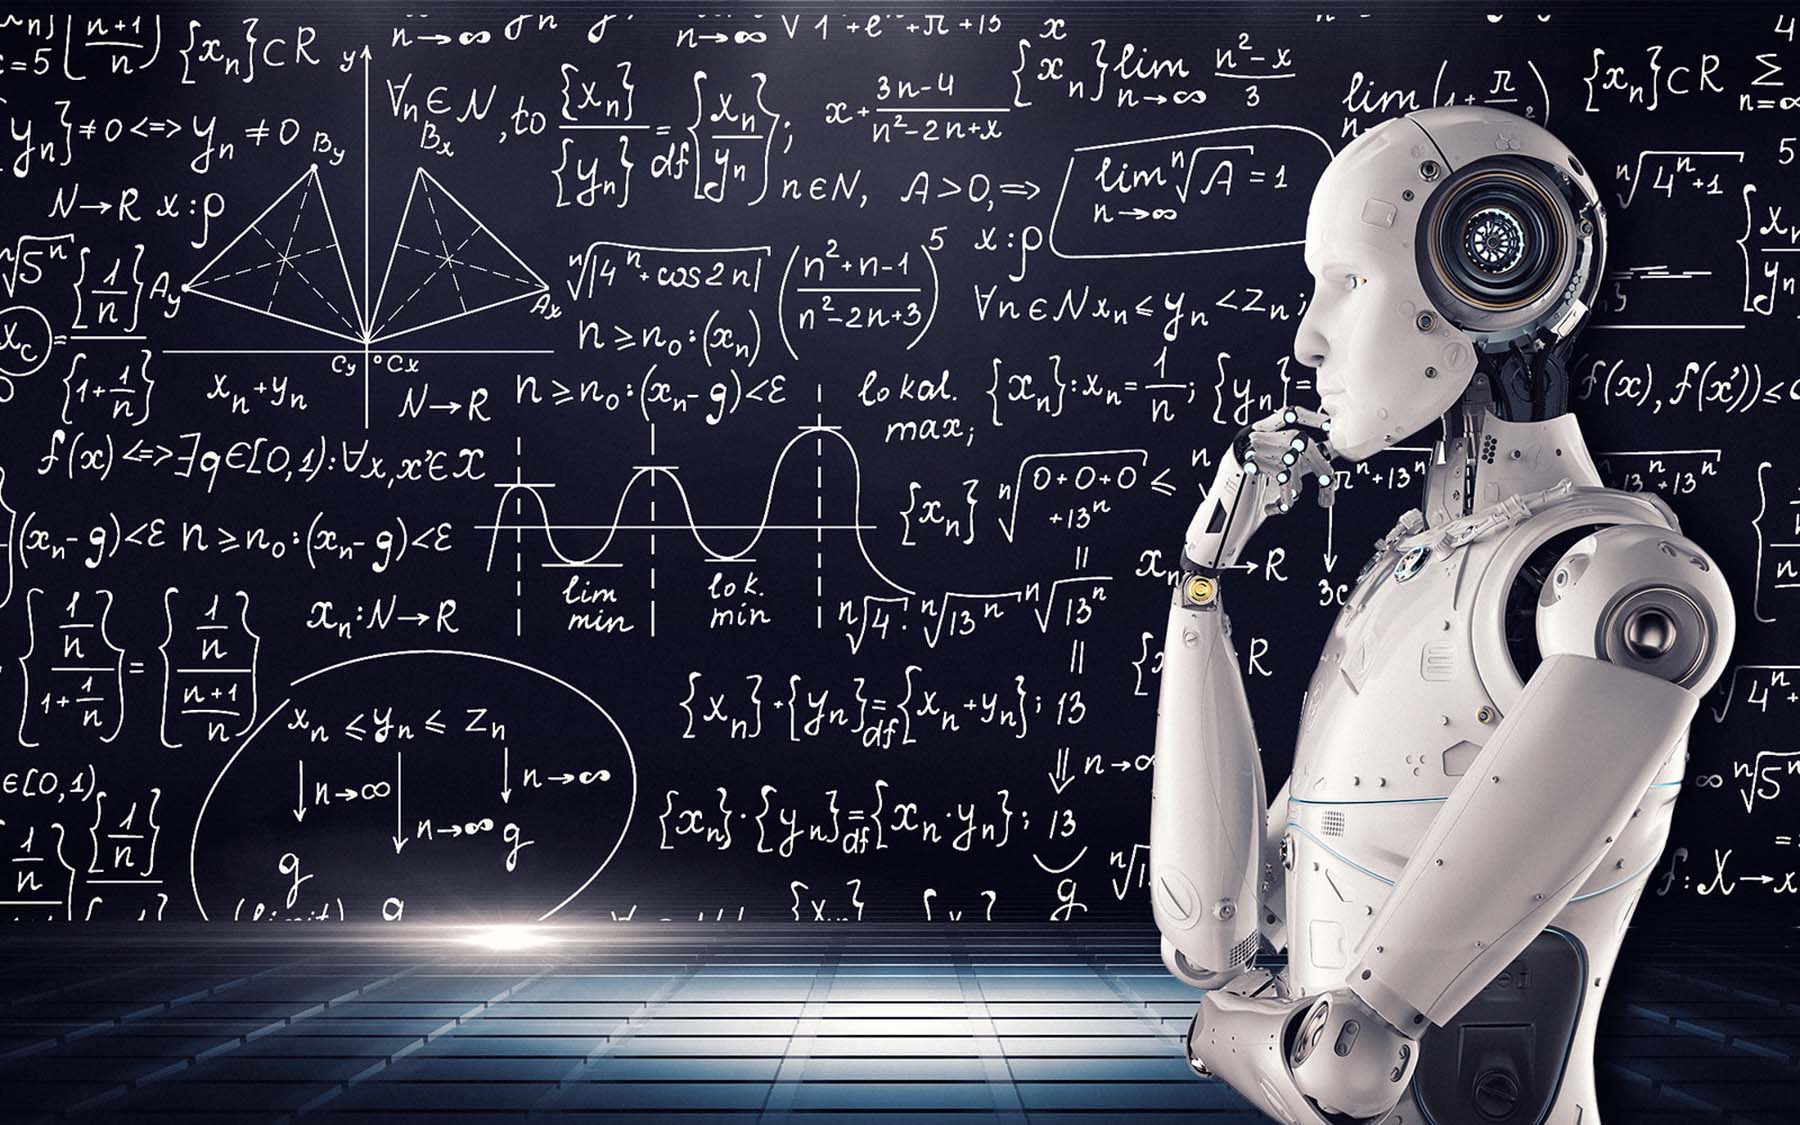
\includegraphics[width=0.8\textwidth]{Figures/AI_Robot-AI-machine-learning-hero.jpg}\\
    智能机器人
  \end{columns}

  \begin{columns}
    \column{0.33\textwidth}
    \centering
    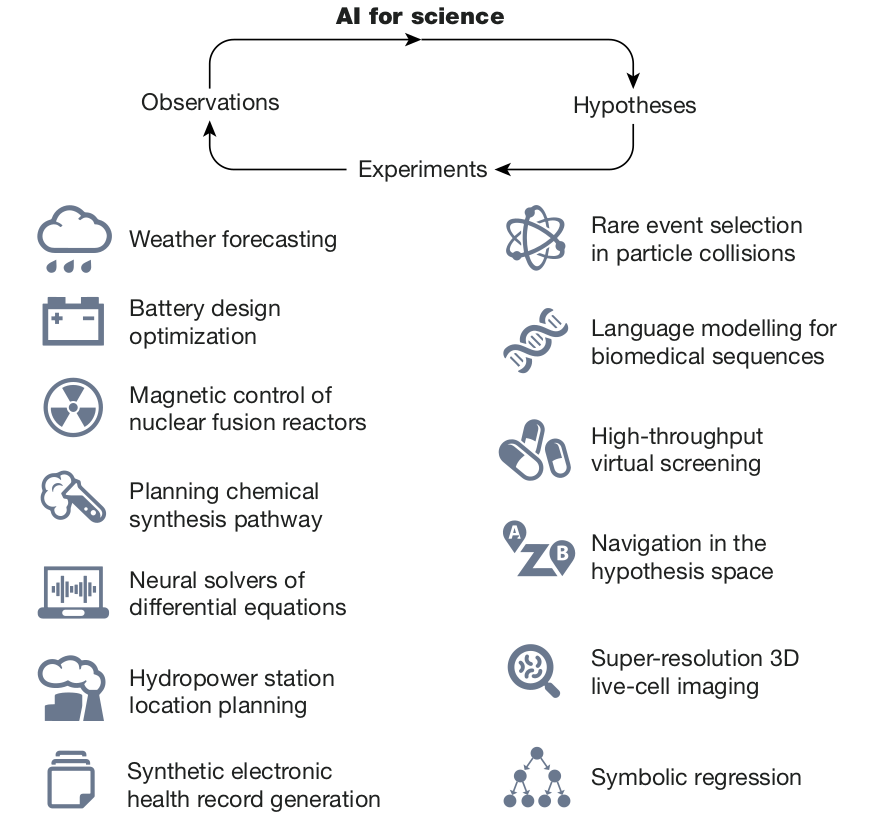
\includegraphics[width=0.8\textwidth]{Figures/AI_for_Science-1.png}

    \column{0.33\textwidth}
    \centering
    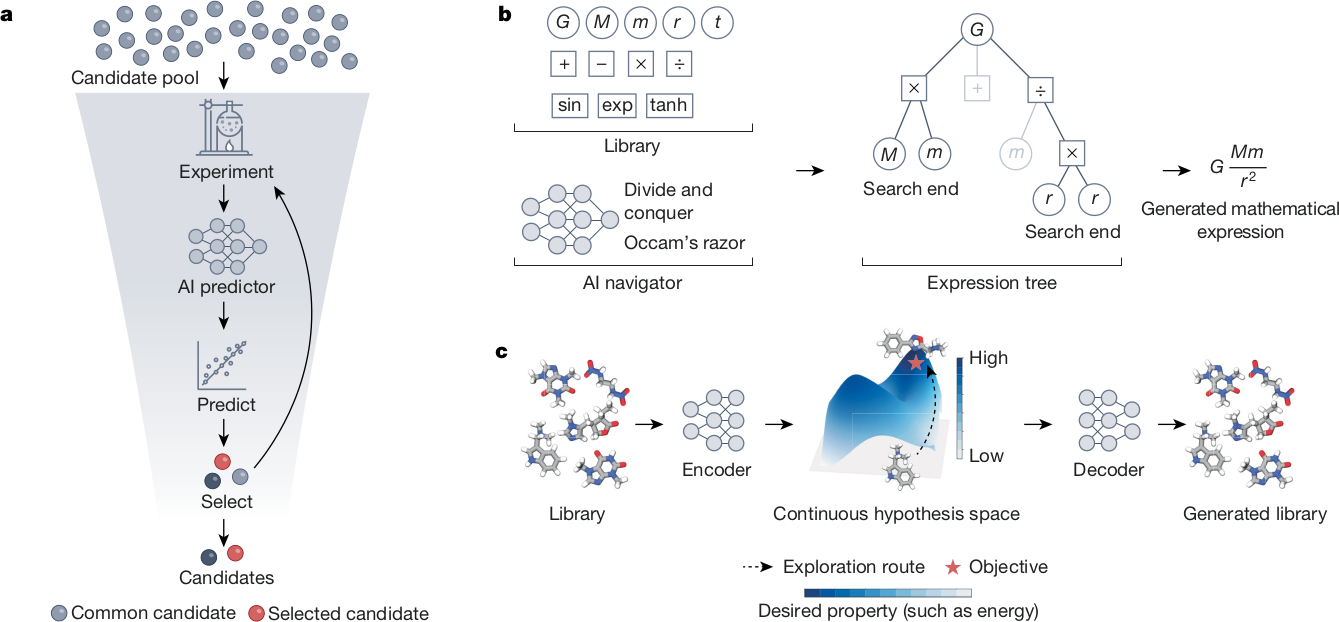
\includegraphics[width=0.8\textwidth]{Figures/AI_for_Science-3.jpeg}\\
    \textcolor{red}{\textrm{AI for Science}}

    \column{0.33\textwidth}
    \centering
    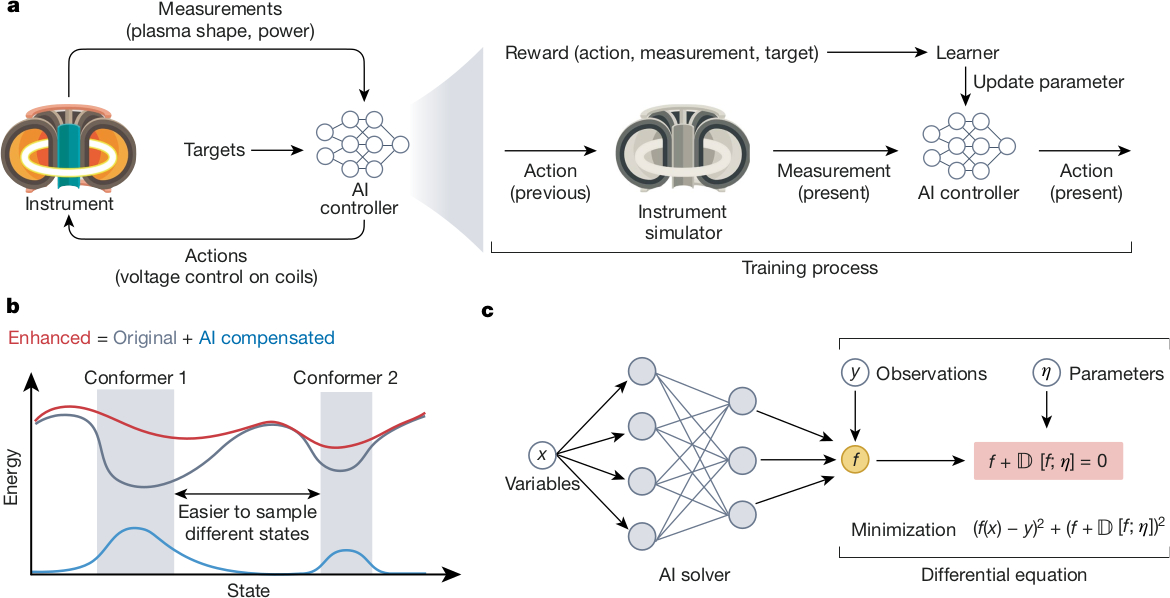
\includegraphics[width=0.8\textwidth]{Figures/AI_for_Science-4.jpeg}
  \end{columns}
\end{frame}

%\subsection{伦理与挑战}
%\begin{frame}{值得思考的问题}
%  \begin{alertblock}{伦理挑战}
%    \begin{itemize}
%      \item 算法偏见与公平性
%      \item 隐私保护问题
%      \item 就业市场影响
%      \item 自主武器系统
%    \end{itemize}
%  \end{alertblock}
%
%  \begin{exampleblock}{未来展望}
%    人类与AI协同发展
%  \end{exampleblock}
%\end{frame}

\section{材料基因工程简介}
\frame
{
	\frametitle{科学研究的范式变更}
\begin{figure}[h!]
\vspace*{-0.28in}
\centering
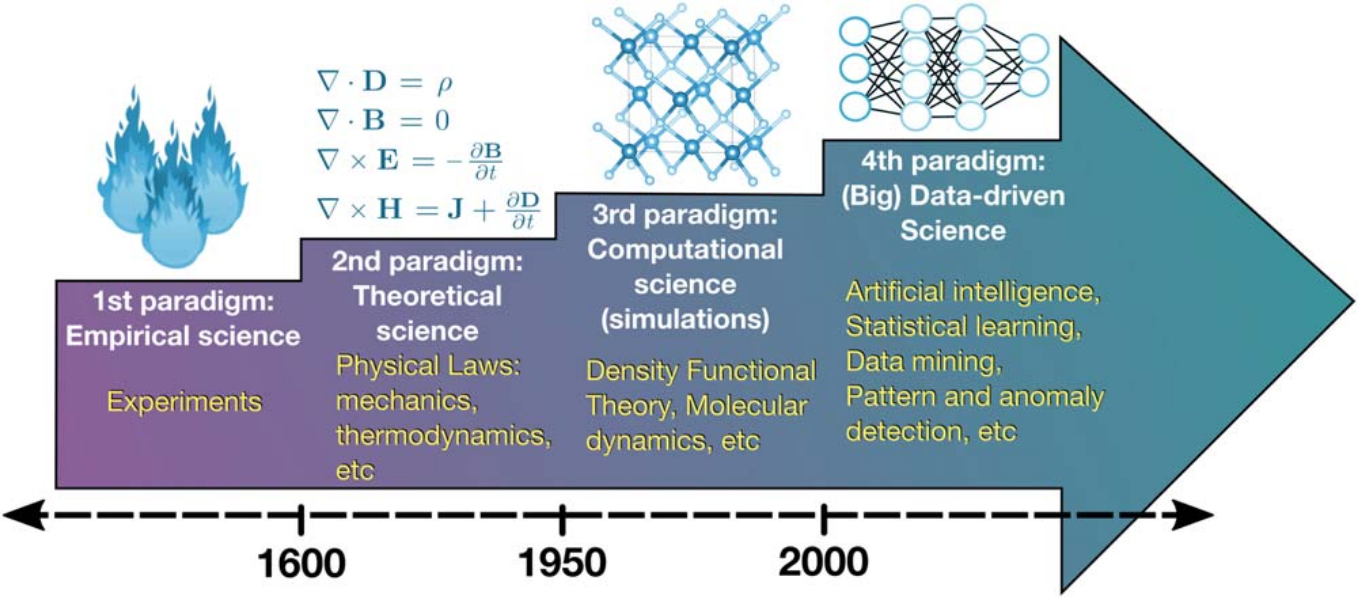
\includegraphics[height=2.00in,width=4.15in]{Figures/Four_Model_3.png}
%\caption{\tiny \textrm{Pseudopotential for metallic sodium, based on the empty core model and screened by the Thomas-Fermi dielectric function.}}%(与文献\cite{EPJB33-47_2003}图1对比)
\label{Four_Model}
\end{figure}
\begin{minipage}[b]{0.48\textwidth}
 {\fontsize{7.5pt}{6.0pt}\selectfont\begin{itemize}%[+-| alert@+>]
	 \setlength{\itemsep}{10pt}
 \item 逐步趋于理性
 \item 逐步趋于复杂
 \end{itemize}}
\end{minipage}
\hfill
\begin{minipage}[b]{0.48\textwidth}
 {\fontsize{7.5pt}{6.0pt}\selectfont\begin{itemize}%[+-| alert@+>]
	 \setlength{\itemsep}{10pt}
 \item 逐步趋于抽象
 \item 逐步趋于深刻
 \end{itemize}}
\end{minipage}
}

\begin{frame}{科学研究的重要助手:~计算模拟}
\begin{figure}[h!]
\vspace*{-0.18in}
\centering
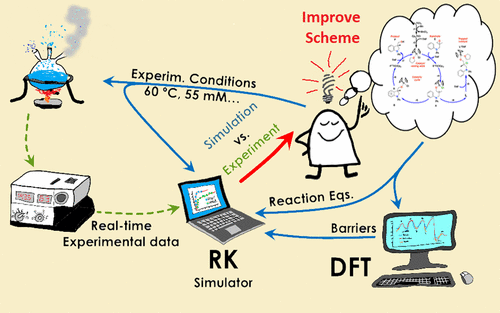
\includegraphics[height=2.55in,width=4.05in]{Figures/Schematic_Material-Design.png}
%\caption{\tiny \textrm{Pseudopotential for metallic sodium, based on the empty core model and screened by the Thomas-Fermi dielectric function.}}%(与文献\cite{EPJB33-47_2003}图1对比)
%\caption{\tiny \textrm{Pseudopotential for metallic sodium, based on the empty core model and screened by the Thomas-Fermi dielectric function.}}%(与文献\cite{EPJB33-47_2003}图1对比)
\label{Schematic_Material-Design}
\end{figure}
\end{frame}

\frame
{
	\frametitle{材料模拟的基本思想和方法}
\begin{figure}[h!]
\vspace*{-0.25in}
\centering
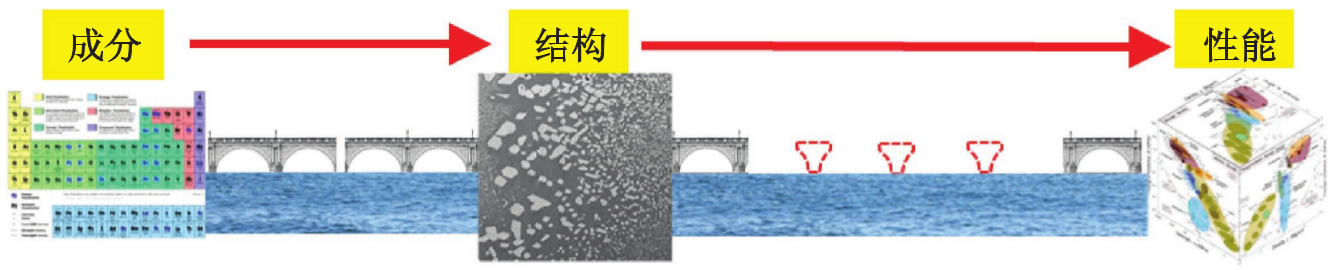
\includegraphics[height=0.80in,width=4.05in]{Figures/MGE-2.png}
%\caption{\tiny \textrm{Pseudopotential for metallic sodium, based on the empty core model and screened by the Thomas-Fermi dielectric function.}}%(与文献\cite{EPJB33-47_2003}图1对比)
\label{MGE}
\end{figure}
\begin{minipage}[c]{0.30\textwidth}
\begin{itemize}%[+-| alert@+>]
\vspace*{-2.25in}
 {\fontsize{7.5pt}{6.0pt}\selectfont
	 \setlength{\itemsep}{10pt}
 \item 变革研发模式,计算-实验-理论-数据科学相融合: 高效、低耗按需设计
 \item 数据驱动的材料创新平台主要面向复杂材料的模拟}
 \end{itemize}
\end{minipage}
\hfill
\begin{minipage}[b]{0.68\textwidth}
\begin{figure}[h!]
%\vspace*{-0.25in}
\centering
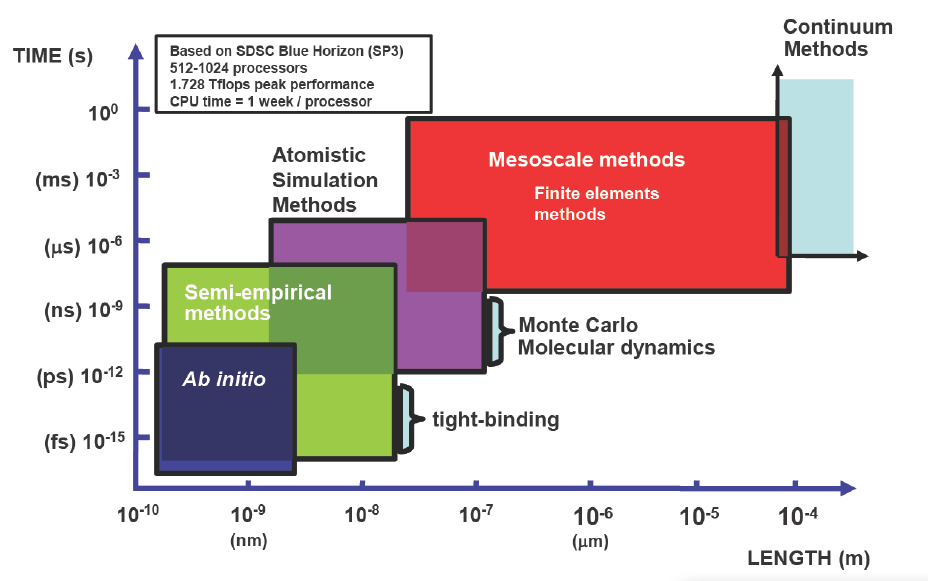
\includegraphics[height=1.60in,width=2.75in]{Figures/Multi-Scale-6.png}
%\caption{\tiny \textrm{Pseudopotential for metallic sodium, based on the empty core model and screened by the Thomas-Fermi dielectric function.}}%(与文献\cite{EPJB33-47_2003}图1对比)
\label{Multi-Scale}
\end{figure}
\end{minipage}
}

\frame
{
	\frametitle{数据驱动的科学研究}
前所未有的计算能力和大规模的数据收集能力%,现代科学正在进入“第四范式”:
\begin{figure}[h!]
%\vspace*{-0.05in}
\centering
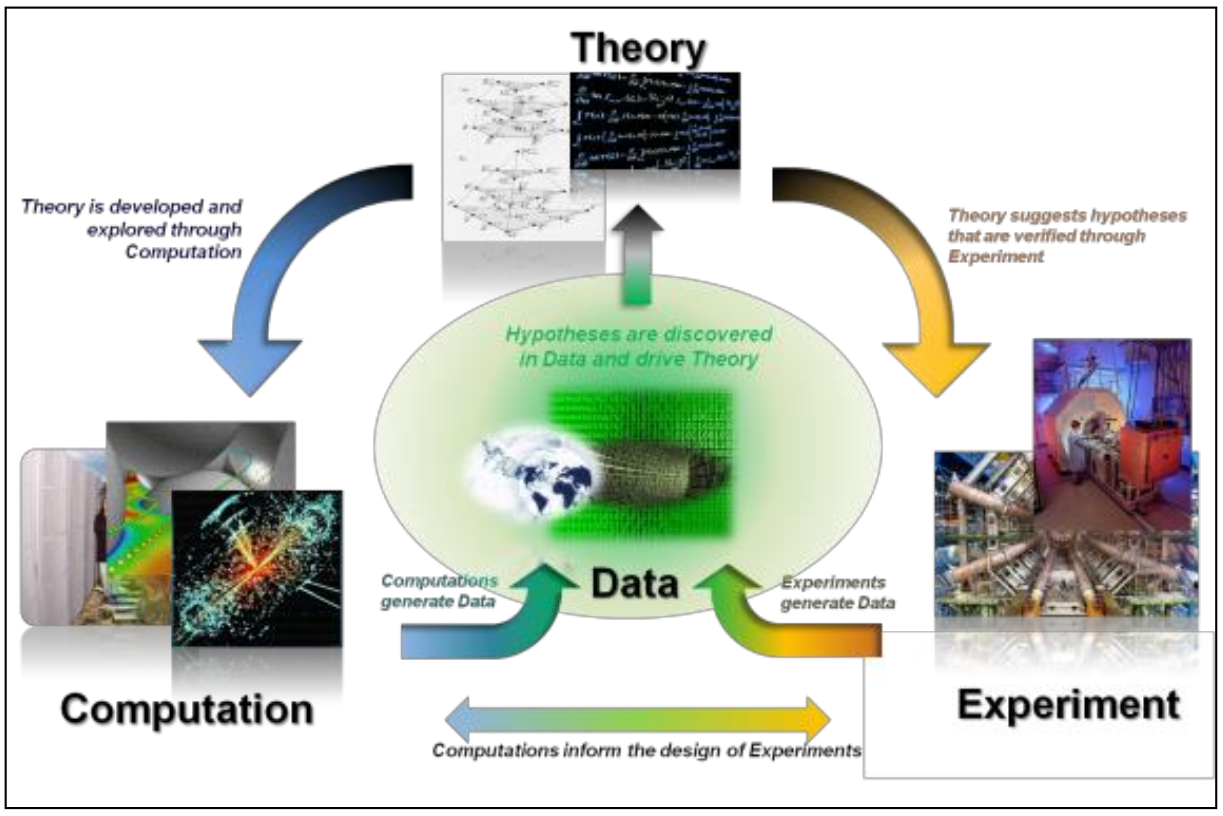
\includegraphics[height=2.40in,width=3.75in]{Figures/Four_Model_1.png}
%\caption{\tiny \textrm{Pseudopotential for metallic sodium, based on the empty core model and screened by the Thomas-Fermi dielectric function.}}%(与文献\cite{EPJB33-47_2003}图1对比)
\label{Four_Model_1}
\end{figure}
科学的新驱动力:~\textcolor{red}{密集数据}+\textcolor{red}{人工智能}\\
}

\frame
{
	\frametitle{\textrm{AI for Science:}~材料学}
\begin{figure}[h!]
\vspace*{-0.18in}
\centering
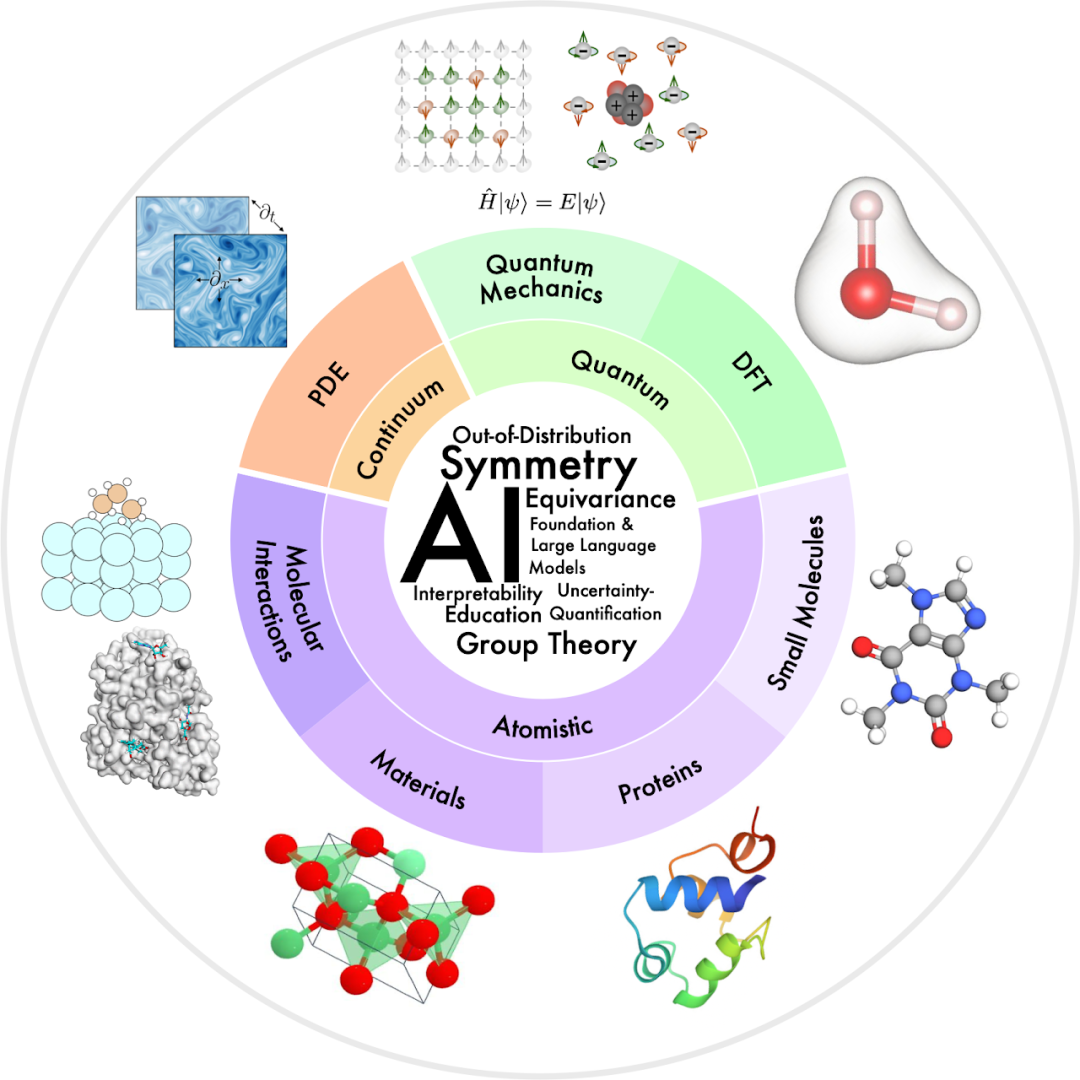
\includegraphics[height=2.95in,width=3.05in]{Figures/AI-for-Science.png}
\label{AI_for_Sciences}
\end{figure}
}

\frame
{
	\frametitle{材料基因工程}
\begin{figure}[h!]
\vspace*{-0.18in}
\centering
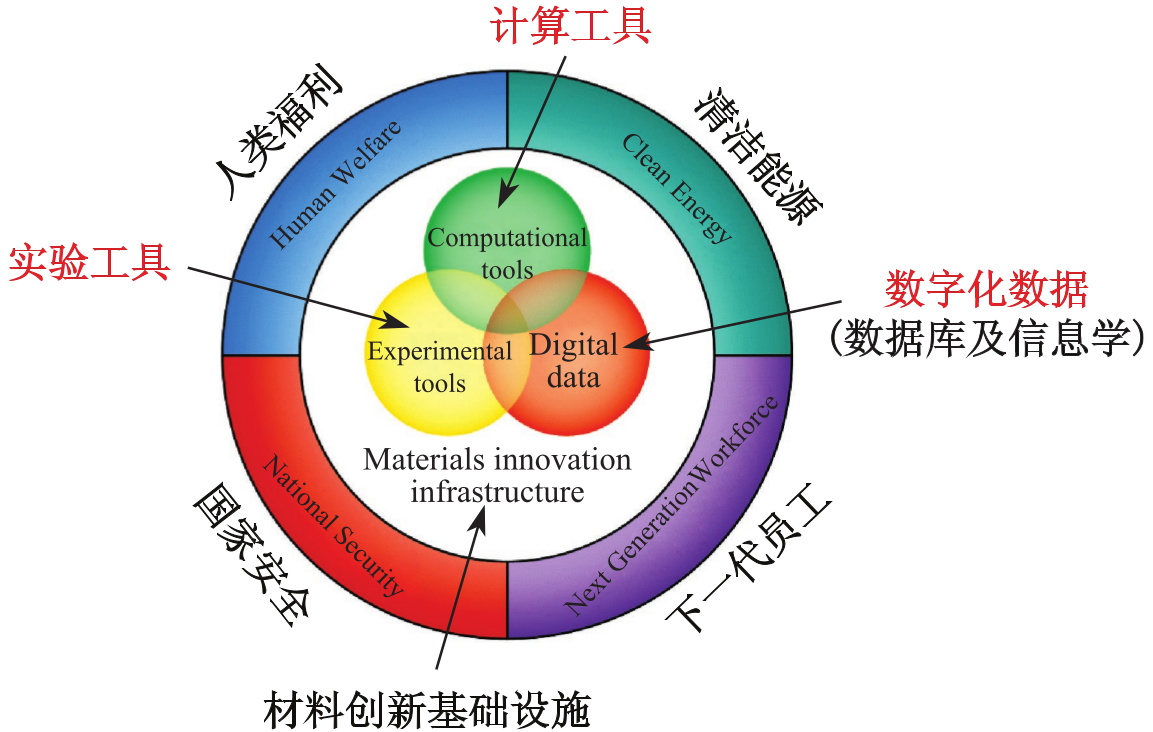
\includegraphics[height=2.55in,width=4.05in]{Figures/MGE.png}
%\caption{\tiny \textrm{Pseudopotential for metallic sodium, based on the empty core model and screened by the Thomas-Fermi dielectric function.}}%(与文献\cite{EPJB33-47_2003}图1对比)
%\caption{\tiny \textrm{Pseudopotential for metallic sodium, based on the empty core model and screened by the Thomas-Fermi dielectric function.}}%(与文献\cite{EPJB33-47_2003}图1对比)
\label{MGE}
\end{figure}
}

\begin{frame}
	\frametitle{材料基因工程推动新材料发展}
\begin{figure}[h!]
\vspace*{-0.25in}
\centering
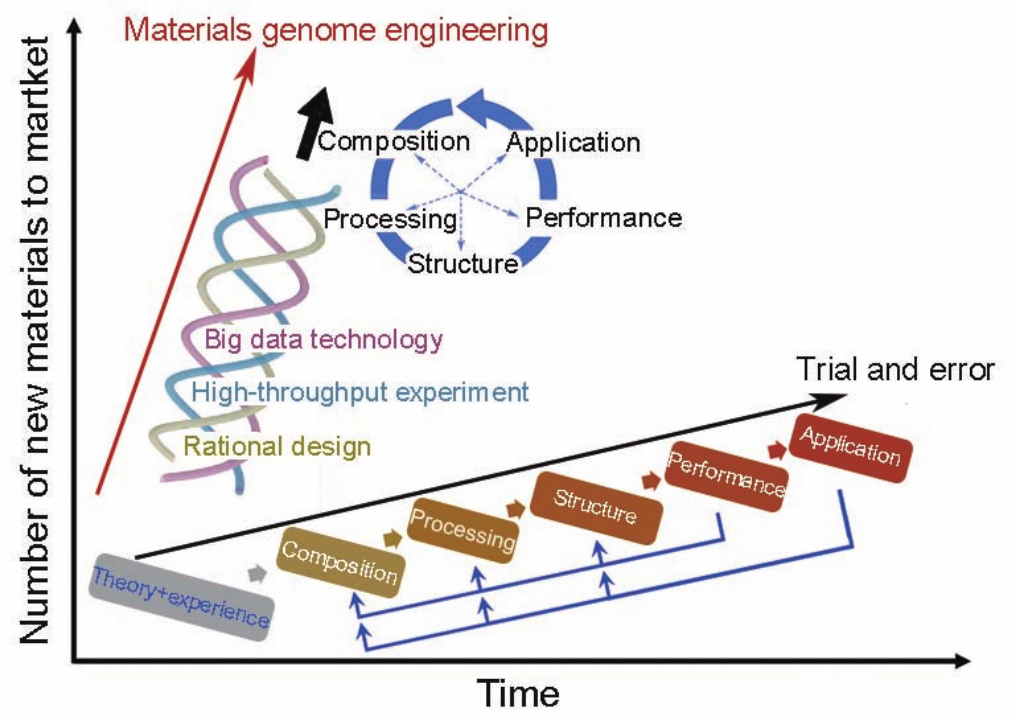
\includegraphics[height=2.90in,width=4.80in,viewport=0 0 1250 710,clip]{Figures/MGE_idea.png}
%\caption{\tiny \textrm{Pseudopotential for metallic sodium, based on the empty core model and screened by the Thomas-Fermi dielectric function.}}%(与文献\cite{EPJB33-47_2003}图1对比)
\label{MGE_idea}
\end{figure}
\end{frame}

\section{数字孪生技术}
\begin{frame}{数字孪生的定义}
	\begin{block}{\textrm{2010}年,\textrm{NASA}定义的数字孪生:~}
		\textcolor{blue}{物理实体}的高保真\textcolor{blue}{数字镜像},通过\textcolor{magenta}{实时数据更新}实现动态仿真
  \end{block}
%
%  \begin{columns}
%    \column{0.6\textwidth}
%    \begin{itemize}
      %\item 
%  三要素:物理实体、数字模型、数据连接
 %     \item
%    \end{itemize}

%    \column{0.4\textwidth}
\begin{figure}[h!]
%\vspace*{0.05in}
\centering
     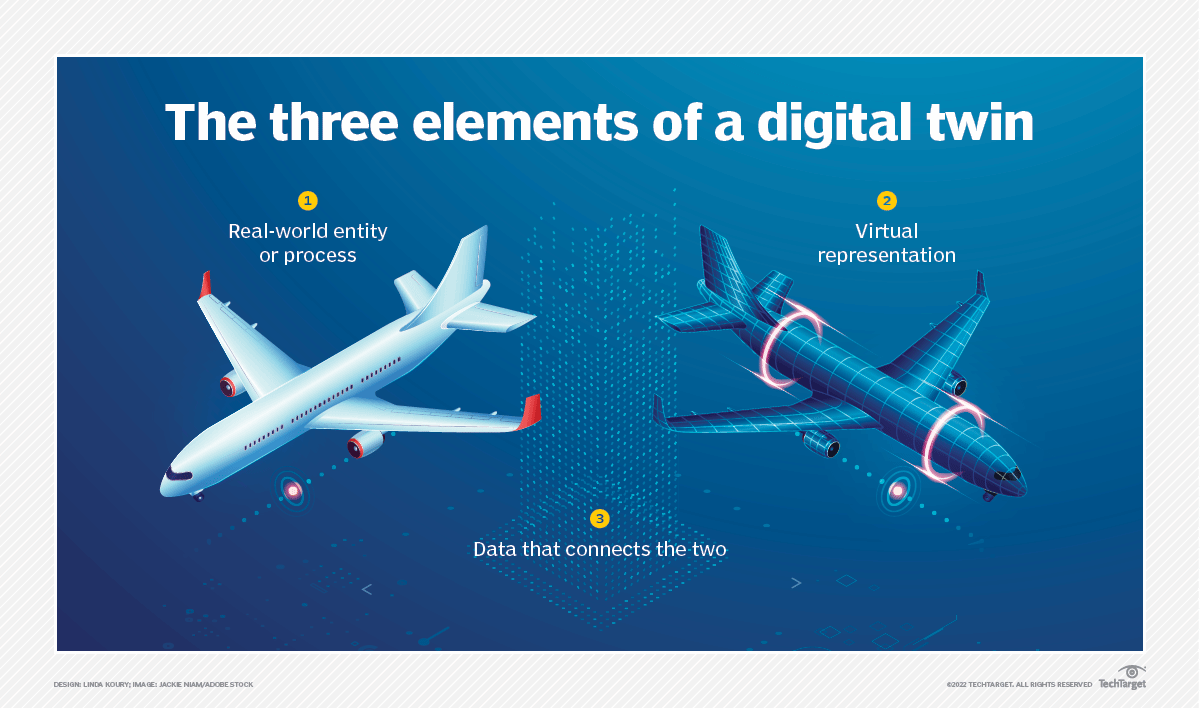
\includegraphics[height=1.6in, width=2.9in, viewport=30 30 1100 680,clip]{Figures/Three-elements_of_a_digital-twin.png}
\caption{\tiny \textrm{All three elements must be present for a true digital twin.}}%(与文献\cite{EPJB33-47_2003}图1对比)
\label{Fig:Three-elements_of_a_digital-twin}
\end{figure}
%  \end{columns}
\textcolor{red}{关键特征}:~
%      \begin{itemize}
 %       \item 
虚实映射、
  %      \item 
实时交互、
   %     \item 
迭代优化
   %   \end{itemize}
\end{frame}

% ========== 发展历程 ==========
\subsection{发展历程}
\begin{frame}{标志性时间节点}
\begin{figure}[h!]
%\vspace*{0.05in}
\centering
     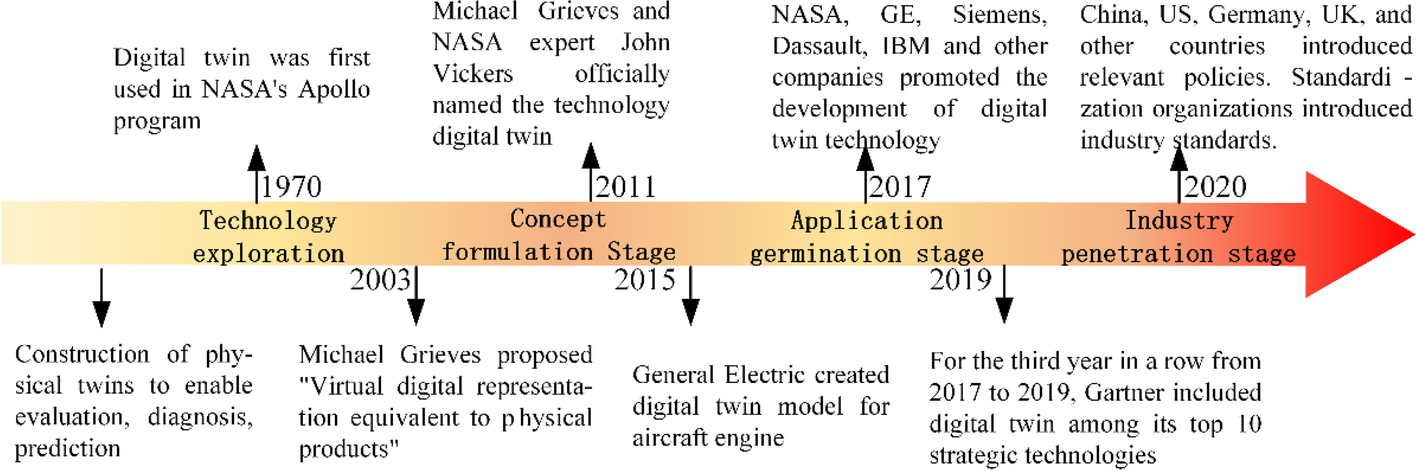
\includegraphics[height=1.2in, width=4.0in, viewport=0 0 1416 471,clip]{Figures/Evolution_of_Digital-Twin.png}
\caption{\tiny \textrm{The evolution of Digital-Twin.}}%(与文献\cite{EPJB33-47_2003}图1对比)
\label{Fig:Evolution_of_Digital-Twin}
\end{figure}
%  \begin{tikzpicture}[overlay, remember picture]
 %   \node[anchor=north east] at (current page.north east) {
 %     \includegraphics[width=0.3\textwidth]{dt_timeline.png}
 %   };
 % \end{tikzpicture}

  \begin{itemize}
	  \item \textrm{2002:~Michigan}大学教授\textrm{M. Grieves}提出``镜像空间模型''
	  \item \textrm{2010:~NASA}将数字孪生应用于航天器健康管理
	  \item \textrm{2017:~GE}推出工业数字孪生平台
	  \item \textrm{2021:~}元宇宙\textrm{(Metaverse)}概念推动数字孪生技术理念的普及
  \end{itemize}
\end{frame}

% ========== 技术架构 ==========
\subsection{技术结构}
%\subsection{系统架构}
\begin{frame}{支撑技术}
\begin{figure}[h!]
\vspace*{-0.15in}
\centering
     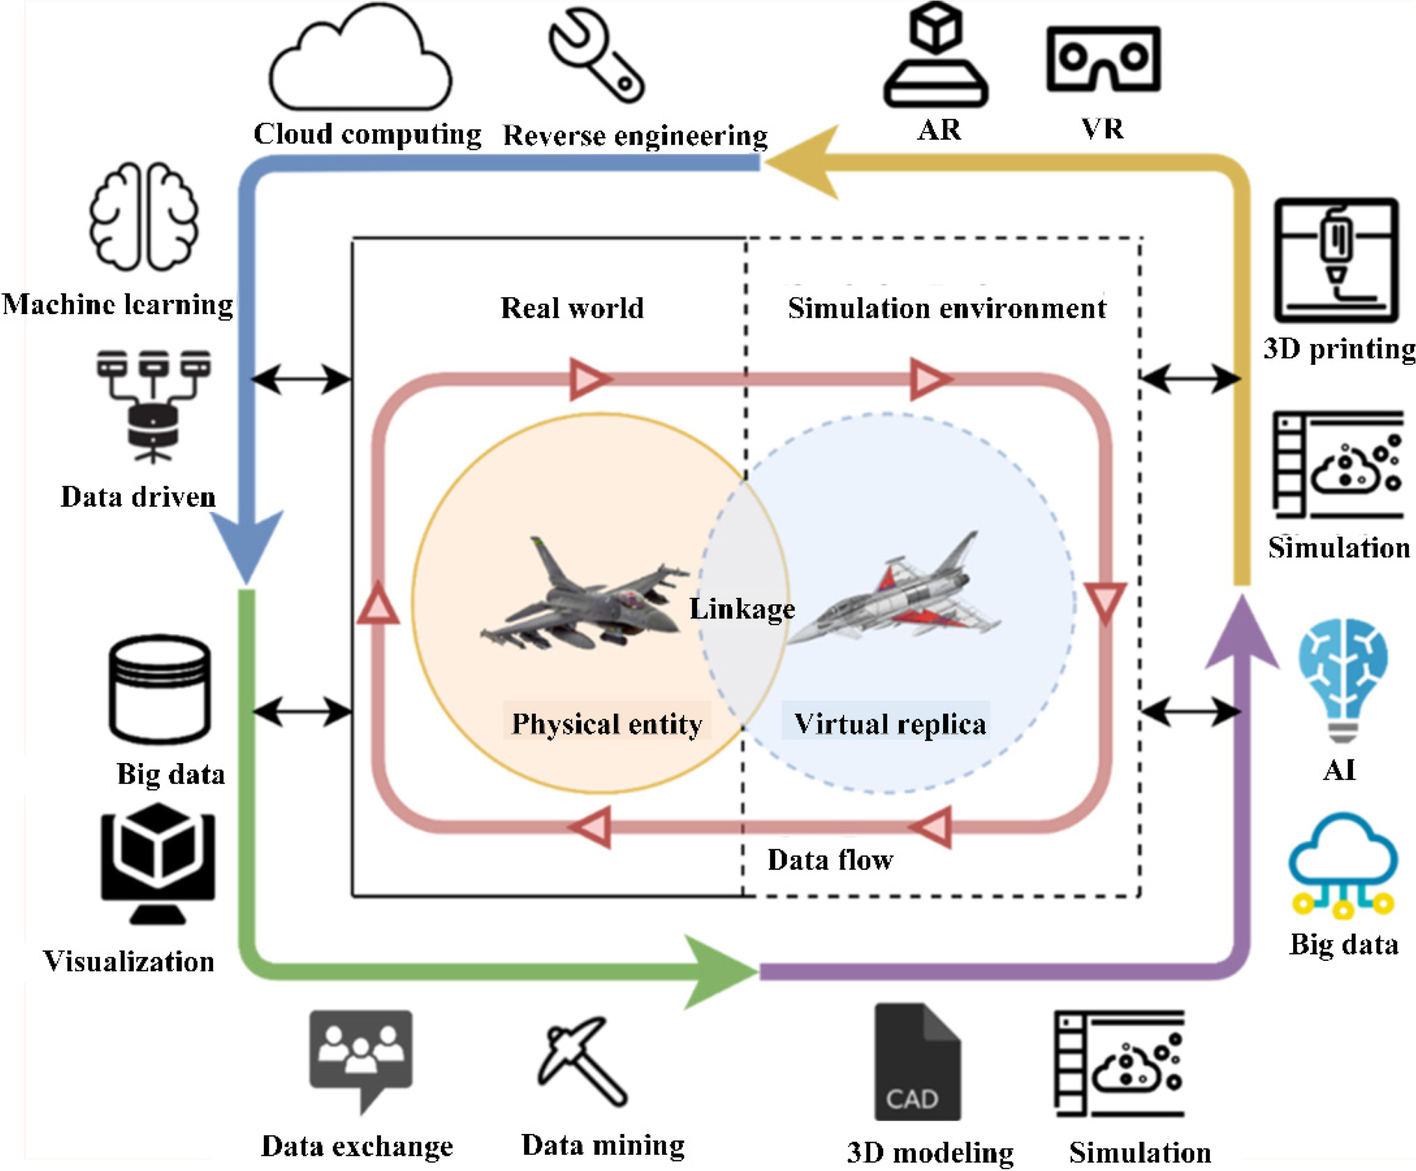
\includegraphics[height=1.8in, width=2.3in, viewport=0 0 1416 1171,clip]{Figures/Digital-Twin_related-technologies.png}
\caption{\tiny \textrm{Digital Twin and the related technologies.}}%(与文献\cite{EPJB33-47_2003}图1对比)
\label{Fig:Digital-Twin_related-technologies}
\end{figure} 
\vspace*{-0.15in}
  \begin{columns}
    \column{0.5\textwidth}
\fontsize{8.2pt}{6.2pt}\selectfont{
    \begin{itemize}
	    \item \textcolor{blue}{物联网\textrm{(IoT)}}:~实时数据采集
      \item \textcolor{magenta}{大数据分析}:~数据价值挖掘
      \item \textcolor{red}{建模仿真}:~\textrm{ANSYS/Matlab}
    \end{itemize}}
    \column{0.5\textwidth}
\fontsize{8.2pt}{6.2pt}\selectfont{
    \begin{itemize}
      \item \textcolor{purple}{\textrm{AI}算法}:~数字模型优化
      \item \textcolor{orange}{云边协同}:~分布式计算
    \end{itemize}}
 %   \includegraphics[width=0.9\textwidth]{dt_tech_stack.png}
 \end{columns}
\end{frame}

\begin{frame}{运行架构:~迭代与升级}
\centering
%\begin{tikzpicture}[
%    box/.style={rectangle,draw,fill=darkgray!20,node distance=1.8cm, text width=15em,text centered,rounded corners,minimum height=2em,thick, auto},
%    arrow/.style={draw,-latex',thick},]
%    \node [box, fill=blue!20, text width=3cm, text centered] (phy) {物理世界\\传感器/设备};
%    \node [box, fill=green!20, below of=phy] (data) {数据层\\\textrm{IoT/5G}传输};
%    \node [box, fill=red!20, below of=data] (model) {数字模型\\仿真引擎/\textrm{AI}算法};
%    \node [box, fill=yellow!20, below of=model] (app) {应用层\\预测/优化/决策};

 \begin{tikzpicture}[box/.style={rectangle,draw, node distance=1.8cm, text centered, auto}]
    \node [box, fill=blue!20, text width=3cm] (phy) {物理世界\\传感器/设备};
    \node [box, fill=green!20, text width=7em, below of=phy] (data) {数据层\\\textrm{IoT/5G}传输};
    \node [box, fill=red!20, text width=9em, below of=data] (model) {数字模型\\仿真引擎/\textrm{AI}算法};
    \node [box, fill=yellow!20, text width=7em, below of=model] (app) {应用层\\预测/优化/决策};
%
    \path[->] (phy) edge (data)
              (data) edge (model)
              (model) edge (app)
              (app.east) edge[bend right=40] node[right] {反向控制} (phy.east);
  \end{tikzpicture}
\end{frame}

%\subsection{关键技术}
% ========== 应用案例 ==========
\subsection{典型应用}
\begin{frame}{智能制造}
	\begin{exampleblock}{\textrm{Siemens factories in Amberg}}

\begin{figure}[h!]
%\vspace*{0.05in}
\centering
     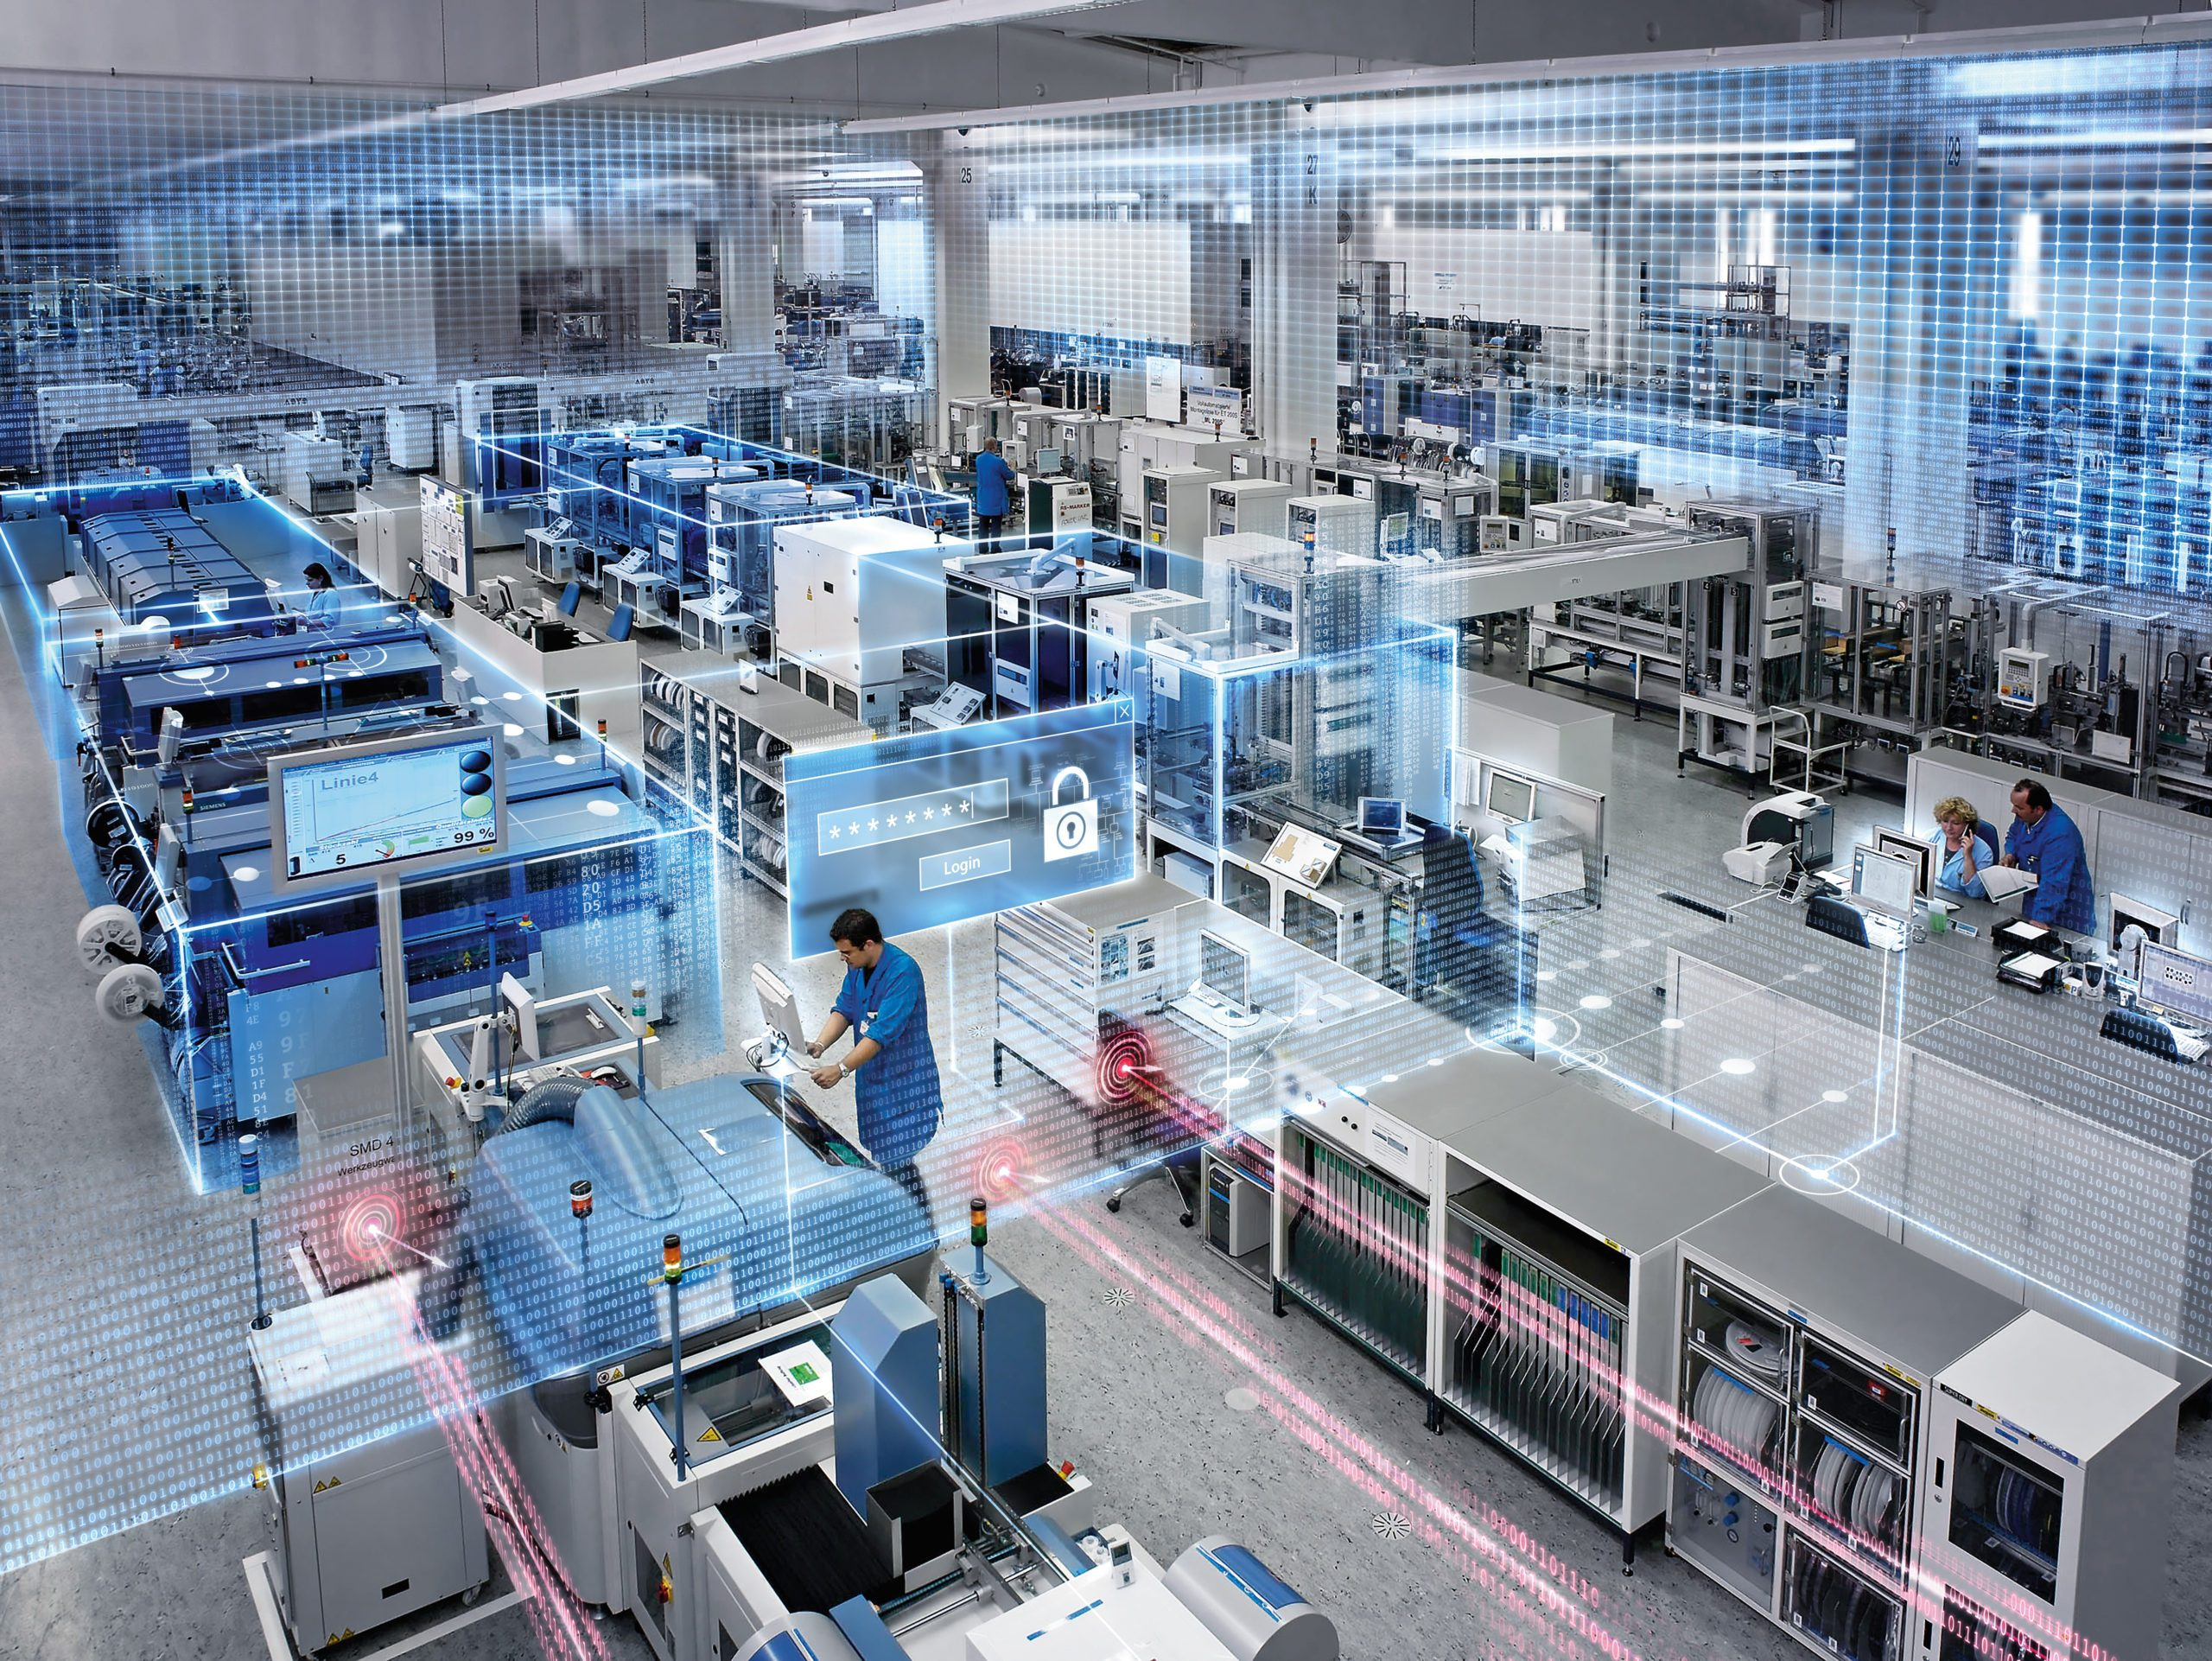
\includegraphics[height=1.8in, width=3.1in, viewport=0 0 2650 1992,clip]{Figures/Siemens_Amberg-Factory.jpeg}
%\caption{\tiny \textrm{All three elements must be present for a true digital twin.}}%(与文献\cite{EPJB33-47_2003}图1对比)
\label{Fig:Siemens_Amberg-Factory}
\end{figure}
  \end{exampleblock}
\fontsize{8.2pt}{6.2pt}\selectfont{
    \begin{itemize}
      \item 生产线数字镜像
      \item 产品全生命周期管理
      \item 故障预测准确率提升\textrm{40\%}
    \end{itemize}}
%  \centering
%  \includegraphics[width=0.6\textwidth]{factory_dt.jpg}
\end{frame}

\begin{frame}{智慧城市}
%  \begin{columns}
 %   \column{0.6\textwidth}
 %   \begin{itemize}
  %    \item 
	城市三维数字模型
\begin{figure}[h!]
%\vspace*{0.05in}
\centering
     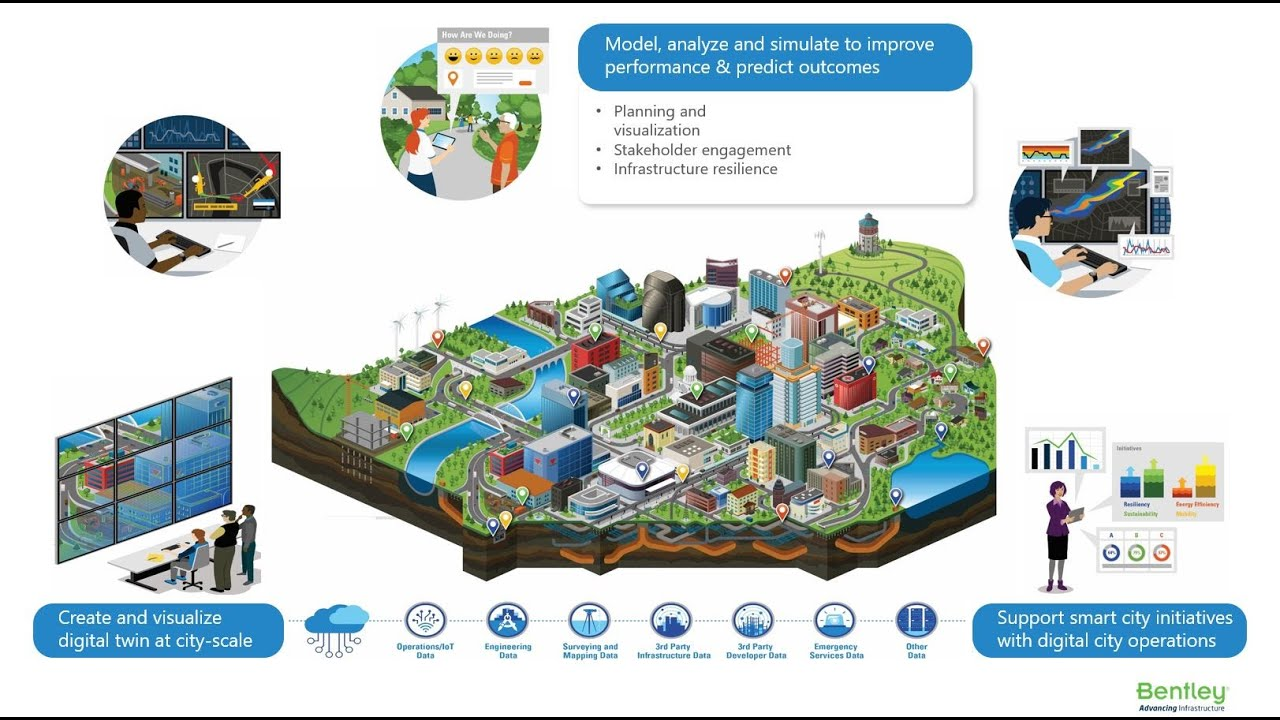
\includegraphics[height=1.5in, width=2.8in, viewport=0 0 1280 720,clip]{Figures/Digital-Twin_Smart-city-infrustruct.jpg}
\caption{\tiny \textrm{Digital Twin for Smart city:~infrustruct.}}%(与文献\cite{EPJB33-47_2003}图1对比)
\label{Fig:Digital-Twin_Smart-city-infrustruct}
\end{figure}
应用场景:
\vskip -10pt
  \begin{columns}
   \column{0.6\textwidth}
\fontsize{8.2pt}{6.2pt}\selectfont{
      \begin{itemize}
        \item 交通流量仿真
        \item 应急演练
\end{itemize}}
  %  \end{itemize}

    \column{0.4\textwidth}
\fontsize{8.2pt}{6.2pt}\selectfont{
   \begin{itemize}
        \item 能源管理
\end{itemize}}
%    \includegraphics[width=\textwidth]{smart_city.png}
  \end{columns}
\end{frame}

\begin{frame}{智慧国家}
%  \begin{columns}
 %   \column{0.6\textwidth}
 %   \begin{itemize}
 %     \item 
	新加坡:~``虚拟新加坡''
\begin{figure}[h!]
%\vspace*{0.05in}
\centering
     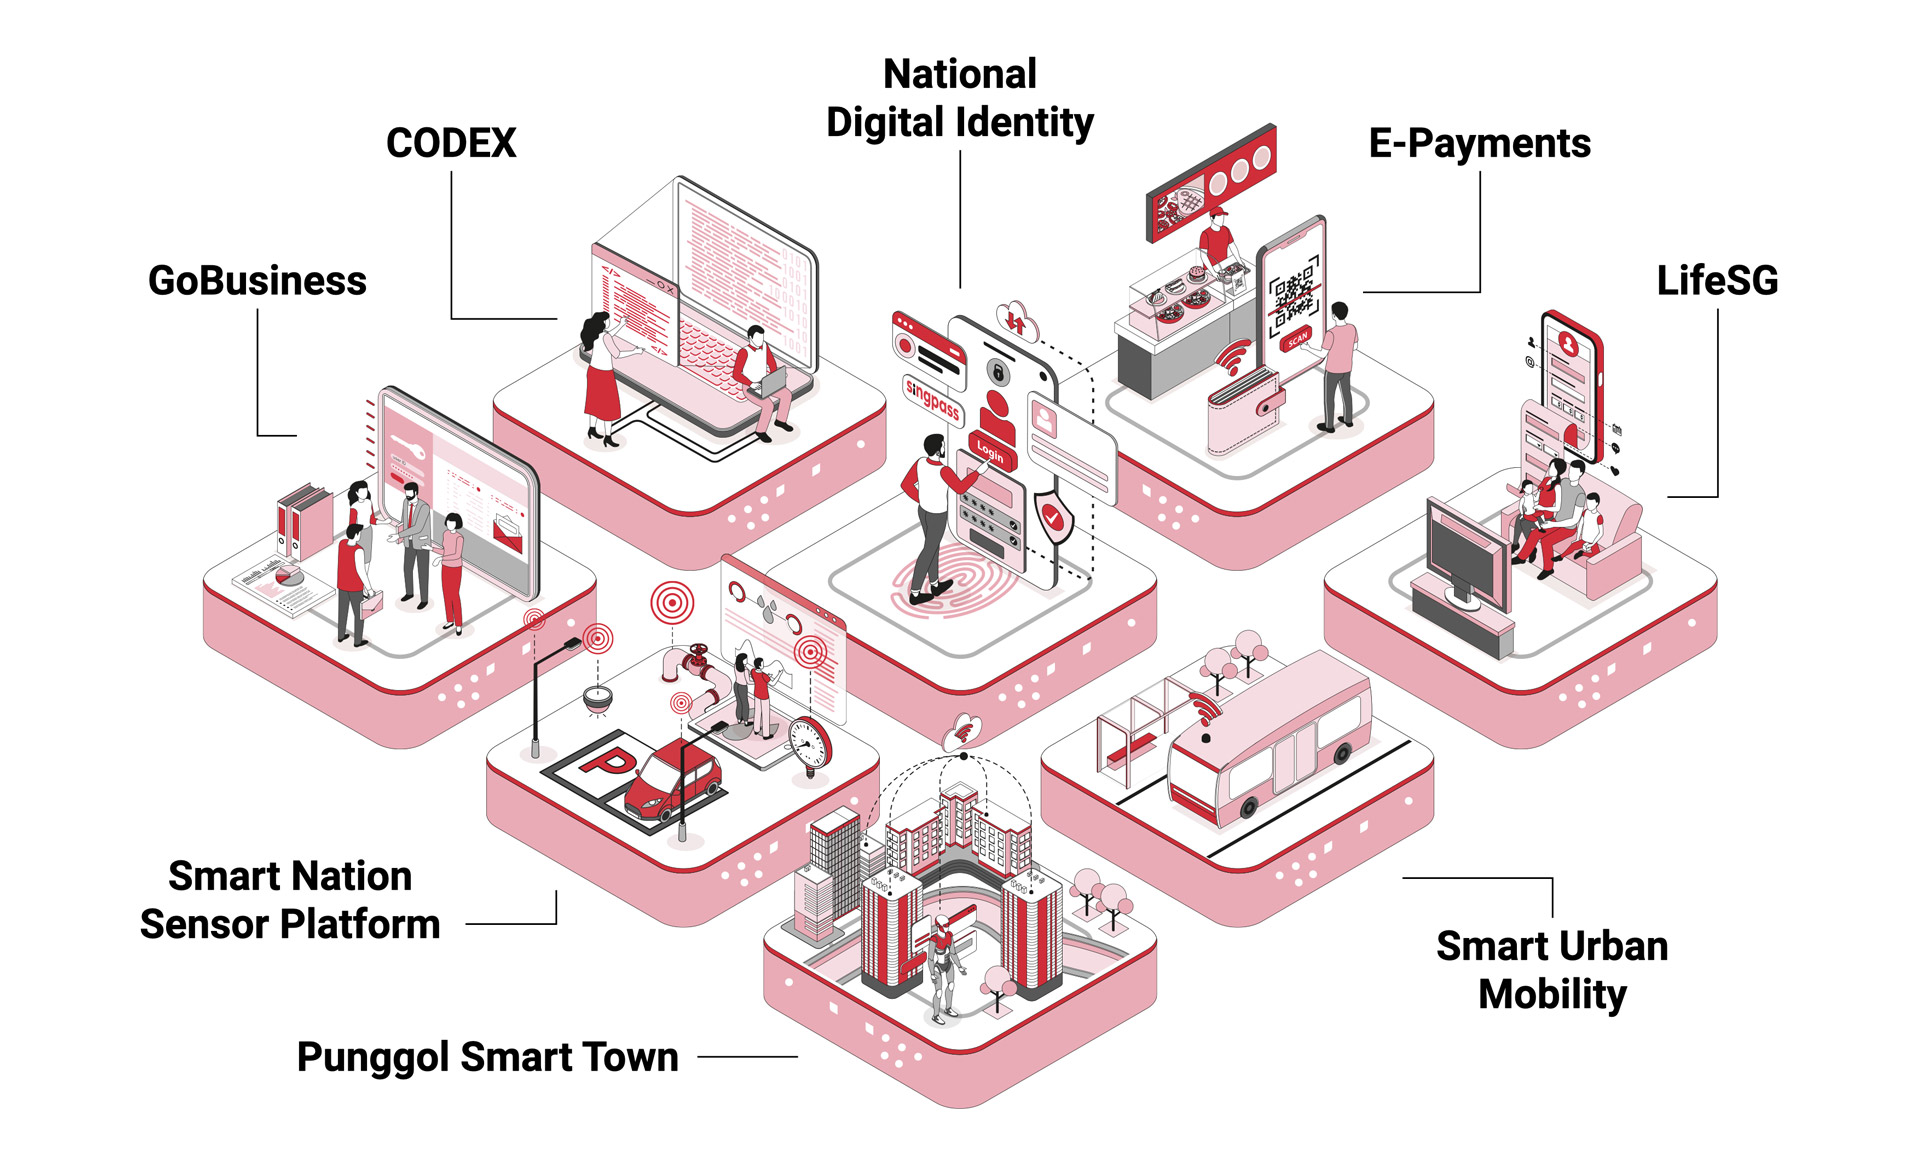
\includegraphics[height=2.4in, width=4.0in, viewport=0 0 1920 1154,clip]{Figures/Smart-city_strategic_national_projects.jpg}
\caption{\tiny \textrm{Smart Nation Singapore (The Smart Nation Digital Government Group).}}%(与文献\cite{EPJB33-47_2003}图1对比)
\label{Fig:Smart-city_strategic_national_projects}
\end{figure}
  %    \item 城市三维数字模型
  %    \item 应用场景:
  %    \begin{itemize}
  %      \item 交通流量仿真
  %      \item 应急演练
  %      \item 能源管理
  %    \end{itemize}
  %  \end{itemize}

  %  \column{0.4\textwidth}
%    \includegraphics[width=\textwidth]{smart_city.png}
%  \end{columns}
\end{frame}

% ========== 挑战与趋势 ==========
%\subsection{未来展望}
%\begin{frame}{技术挑战}
%  \begin{alertblock}{主要瓶颈}
%    \begin{itemize}
%      \item 多源异构数据融合
%      \item 模型精度与计算效率平衡
%      \item 安全与隐私保护
%      \item 标准化体系缺失
%    \end{itemize}
%  \end{alertblock}
%
%  \begin{exampleblock}{发展趋势}
%    \begin{itemize}
%      \item 数字孪生+元宇宙融合
%      \item 自主进化型数字孪生
%      \item 行业SaaS服务平台
%    \end{itemize}
%  \end{exampleblock}
%\end{frame}

% ========== 总结 ==========
%\section*{总结}
\begin{frame}{展望}
%  \centering
%  \begin{tabular}{cl}
%    \toprule
%    \textbf{维度} & \textbf{价值体现} \\
%    \midrule
%    产品研发 & 缩短\textrm{50\%}以上开发周期 \\
%    生产运营 & 降低\textrm{30\%}运维成本 \\
%    决策支持 & 提升\textrm{80\%}模拟预测精度 \\
%    创新生态 & 构建协同创新平台 \\
%    \bottomrule
%  \end{tabular}
  \centering
  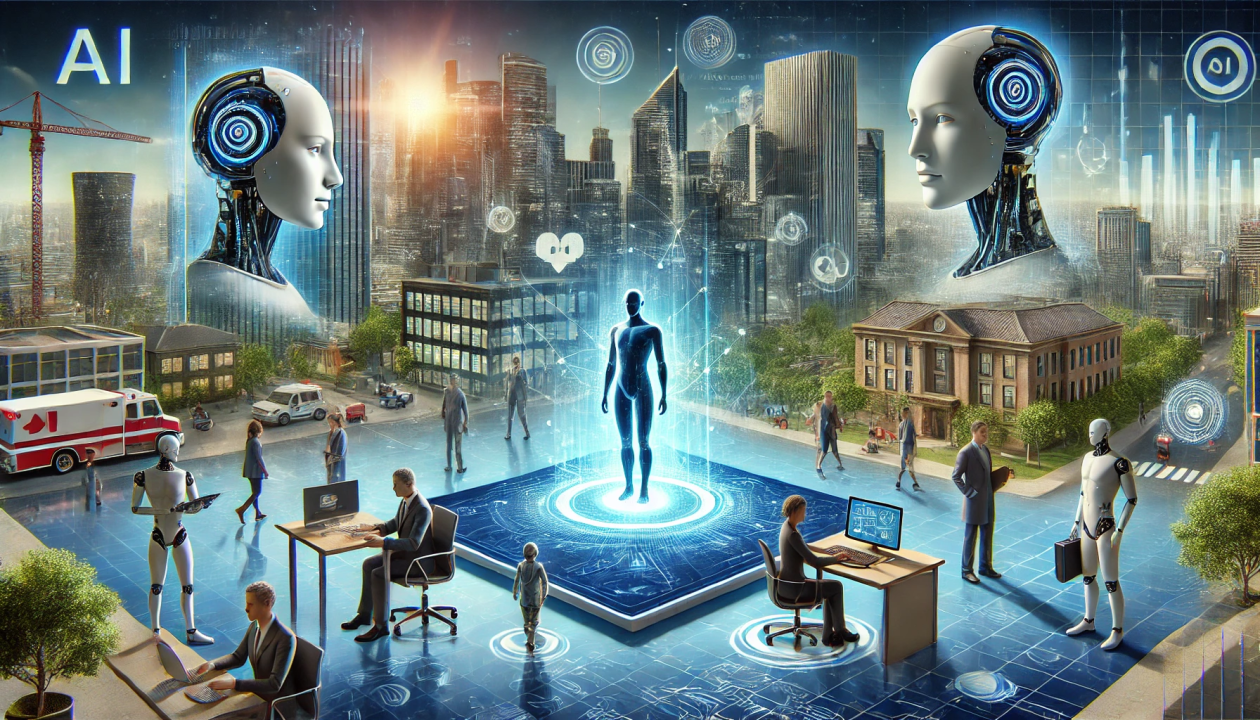
\includegraphics[width=1.0\textwidth]{Figures/Future-of-AI_Agents.png}
  \vskip 8pt
  \textcolor{blue}{\Large 虚实交融,智创未来}
\end{frame}
%
%\begin{frame}{Q\&A}
%  \centering
%  \includegraphics[width=0.7\textwidth]{dt_future.jpg}

%  \begin{footnotesize}
%    图片来源:数字孪生典型应用场景示意图
%  \end{footnotesize}
%\end{frame}

%\appendix
%------------------------------------------------------------------------Reference----------------------------------------------------------------------------------------------
%		\frame[allowframebreaks]{
%\begin{thebibliography}{99}
%\frametitle{主要参考文献}
%{\tiny
%%	\bibitem{PhysCN40-477_2011}曹则贤, \textit{Secular,equation}, \textit{物理}, \textbf{40} \textrm{(2011), 477}
%	\bibitem{PR136-B864_1964}\textrm{P. Hohenberg and W. Kohn, \textit{Phys. Rev.} \textbf{136} (1964), B864}
%	\bibitem{PR140-A1133_1965}\textrm{W. Kohn and L.J. Sham, \textit{Phys. Rev.} \textbf{140} (1965), A1133}
%	\bibitem{JPC12-4409_1979}\textrm{J. Ihm, A. Zunger and L. Cohen, {\textit{J. Phys. C}} \textbf{12} (1979), 4409}
%	\bibitem{PRB41-7892_1990}\textrm{D. Vanderbilt. \textit{Phys. Rev.} B, \textbf{41} (1990), 7892} 
%	\bibitem{JPCM6-8245_1994}\textrm{G. Kresse and J. Hafner. J. Phys: \textit{Condens. Matter}, \textbf{6} (1994), 8245}
%	\bibitem{PRB50-17953_1994}\textrm{P. E. Bl\"ochl. \textit{Phys. Rev.} B, \textbf{50} (1994), 17953}
%	\bibitem{PRB59-1758_1999}\textrm{G. Kresse and D. Joubert \textit{Phys. Rev.} B, \textbf{59} (1999), 1758}
%	\bibitem{PRB12-3060_1975}\textrm{O. K. Andersen. \textit{Phys. Rev.} B, \textbf{12} (1975), 3060}
%	\bibitem{JMP22-2433_1981}\textrm{M. Weiner. \textit{J. Math. Phys.}, \textbf{22} (1981), 2433}
%	\bibitem{PRB26-4571_1982}\textrm{M. Weinert, E. Wimmer and A. J. Freeman. \textit{Phys. Rev.} B, \textbf{26} (1982), 4571}
%	\bibitem{Andersen_Book}\textrm{O. K. Andersen. \textit{Computational Methods in Band Theory} (Plenum, New York, USA, 1971)}
%        \bibitem{Singh}\textrm{D. J. Singh. \textit{Plane Wave, PseudoPotential and the LAPW method} (Kluwer Academic, Boston,USA, 1994)}					%
%	\bibitem{Singh}\textrm{D. J. Singh. \textit{Plane Wave, PseudoPotential and the LAPW method} (Kluwer Academic, Boston,USA, 1994)}
%	\bibitem{Xie-Lu}谢希德、陆栋\:主编, {\textit{固体能带理论}}\:复旦大学出版社, 上海, 1998
%	\bibitem{Nemoshkalenko-Antonov}\textrm{V. V. Nemoshkalenko and V. N. Antonov. \textit{Computational Methods in Solid State Physics} (Gordon and Breach Science Publisher, Amsterdam, The Netherlands, 1998)}
%	\bibitem{Elect_Stru}\textrm{Richard. M. Martin. \textit{Electronic Structure: Basic Theory and Practical Methods} (Cambridge University Press, Cambridge, England, 2004)}
%	\bibitem{Xu_Li_Wang}徐光宪、黎乐民、王德民, {\textit{量子化学——基本原理和从头计算法}}\;\textrm{({\textit{上、中}})}\:科学出版社, 北京, 1980
%%	\bibitem{SSC114-15_2000}\textrm{E. Sj\"ostedt, L. Nordstr\"om and D. J. Singh. \textit{Solid State Commun.}, \textbf{114} (2000), 15}
%}
%\end{thebibliography}
%\nocite*{}
%}
